\chapter{Resultados}

\section{Estatísticas e análises gráficas}

A partir dos dados obtidos do GTFS, dos dados de passageiros disponibilizados pela prefeitura e dos dados do Censo de 2022, do IBGE, podemos criar algumas visualizações gráficas simples, para nos auxiliar a entender as mudanças que ocorreram ao longo do tempo e as possiveis associações que podemos fazer juntando essas 3 bases de dados.

\subsection{Quantidade de linhas e paradas ao longo do tempo
}

Inicialmente, podemos visualizar qual a quantidade de paradas e rotas únicas nas bases do GTFS ao longo do tempo.

\begin{figure}[H]
    \centering
    {%
        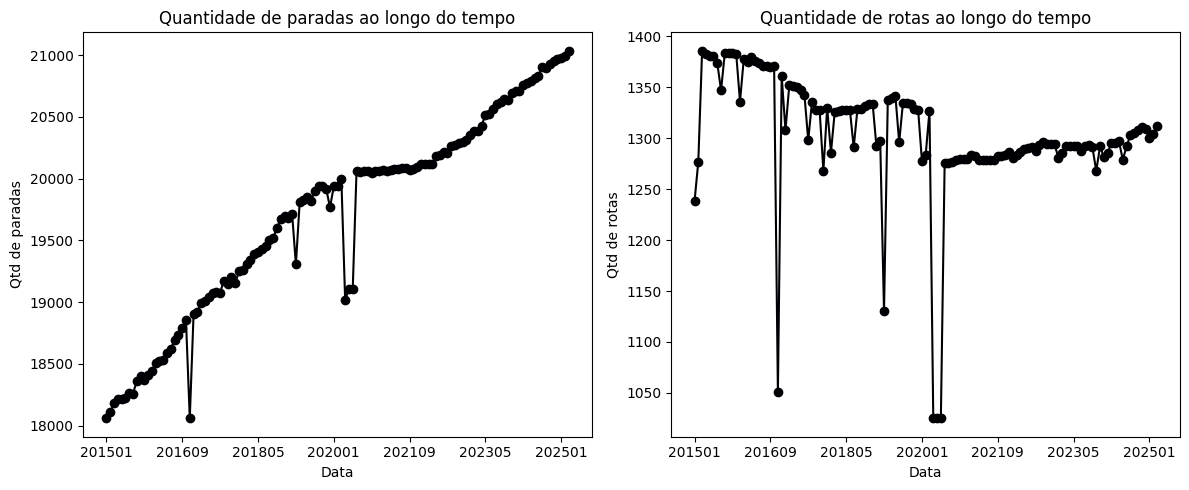
\includegraphics[width=1\textwidth]{figuras/rotas e paradas/qtd de paradas e rotas ao longo do tempo.png}
    }
    \caption{Histórico da quantidade única de rotas e paradas ao longo do tempo. Fonte: A própria autora. }
    \label{grafico_historico_rotas_paradas}
    
\end{figure}
Conseguimos observar um crescimento contínuo no número de paradas, indicando que, mês a mês, a quantidade de locais únicos que o transporte cobre aumenta, o que pode ter sido causado por novas linhas ou pela expansão de linhas já existentes. Já a quantidade de rotas tinha uma tendência decrescente até 2020, e levemente crescente a partir de 2020, podendo indicar que muitas linhas foram extintas ou reestruturadas, e que mais recentemente o sistema tem se expandido. 

Vale notar que há quedas bruscas na quantidade de rotas em alguns períodos de 2016, 2019 e 2020, indicando possíveis reestruturações temporárias da rede, ou a ausência de dados.

Como temos dados geográficos mais detalhados, podemos analisar as mesmas métricas com segregações por zonas, bairros e estações próximas:

\subsubsection{Divisão por zona}
\begin{figure}[H]
    \centering
    {%
        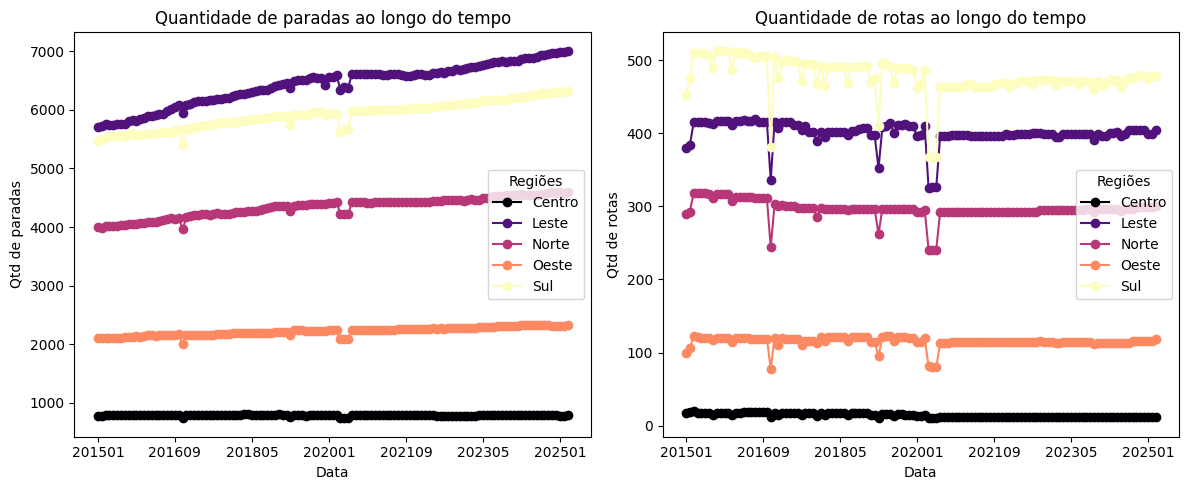
\includegraphics[width=1\textwidth]{figuras/rotas e paradas/qtd de paradas e rotas ao longo do tempo por zona.png}
    }
    \caption{Histórico da quantidade única de rotas e paradas ao longo do tempo por zona. Fonte: A própria autora.}
\end{figure}

Observamos que as regiões Sul e Leste concentram a maior quantidade de paradas e rotas de ônibus, o que reflete a sua extensão territorial e alta demanda populacional. Enquanto o número de paradas cresce de forma contínua em todas as regiões (menos o centro), o número de rotas apresenta pequenas oscilações, com uma queda mais acentuada na região Sul. 

Vale notar que a queda brusca na quantidade de rotas observada no gráfico \ref{grafico_historico_rotas_paradas} não é tão visível no gráfico por zonas, possivelmente por haver rotas que passam por mais de uma região. 

\begin{center}
\begin{minipage}{1\textwidth}
    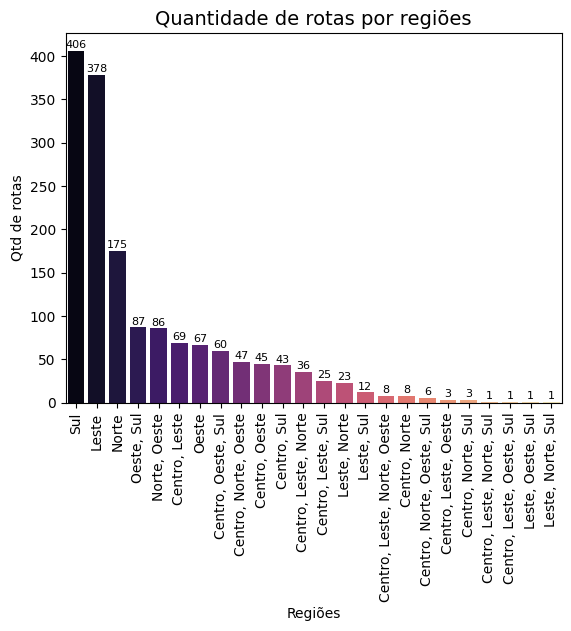
\includegraphics[width=\textwidth]{figuras/rotas e paradas/qtd de rotas por regioes.png}
    \captionof{figure}{Quantidade de rotas por regiões em todo o histórico da base. Fonte: A própria autora.}
   
  
\end{minipage}
\end{center}
% \begin{figure}[H]
%     \centering
%     {%
%         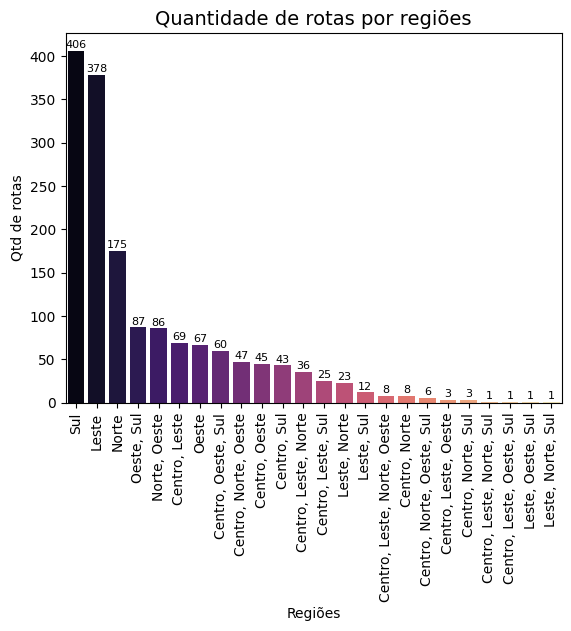
\includegraphics[width=0.8\textwidth]{figuras/rotas e paradas/qtd de rotas por regioes.png}
%     }
%     \caption{Quantidade de rotas por regiões em todo o histórico da base. Fonte: A própria autora. }
    
% \end{figure}
% \FloatBarrier
No gráfico acima, podemos ver que muitas rotas passam por mais de uma região, inclusive, vale notar que a quantidade de rotas que passa exclusivamente pela região Oeste é menor do que a que passa pela Oeste e Norte, e Oeste e Sul. As zonas Sul, Leste e Norte dominam em quantidade de rotas que passam exclusivamente por elas. Também podemos notar que nenhuma rota passa exclusivamente pelo Centro. Dentre as rotas que passam por 4 regiões, a combinação mais comum é Centro, Leste, Norte e Oeste, com 8 rotas.

\subsubsection{Divisão por bairro}

\begin{figure}[H]
    \centering
    
    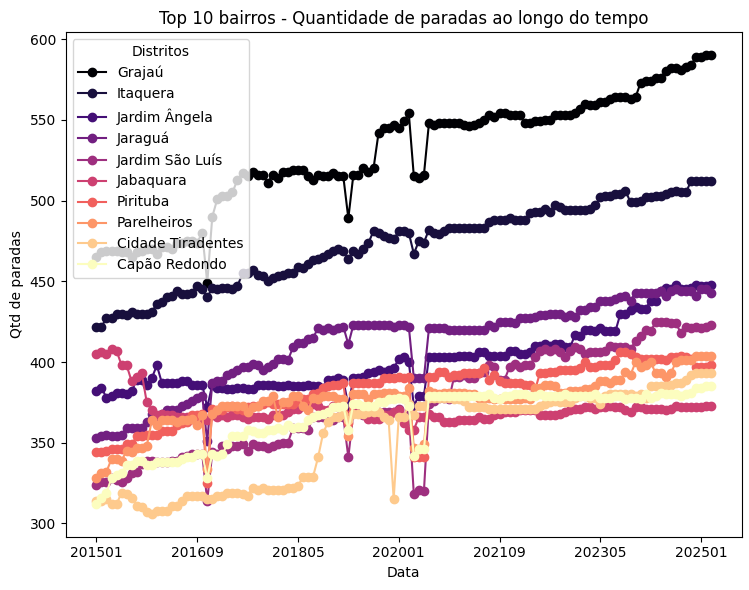
\includegraphics[width=0.75\textwidth]{figuras/rotas e paradas/qtd de rotas e paradas ao longo do tempo por bairro 1.png}
    
    \vspace{0.5cm}
    
    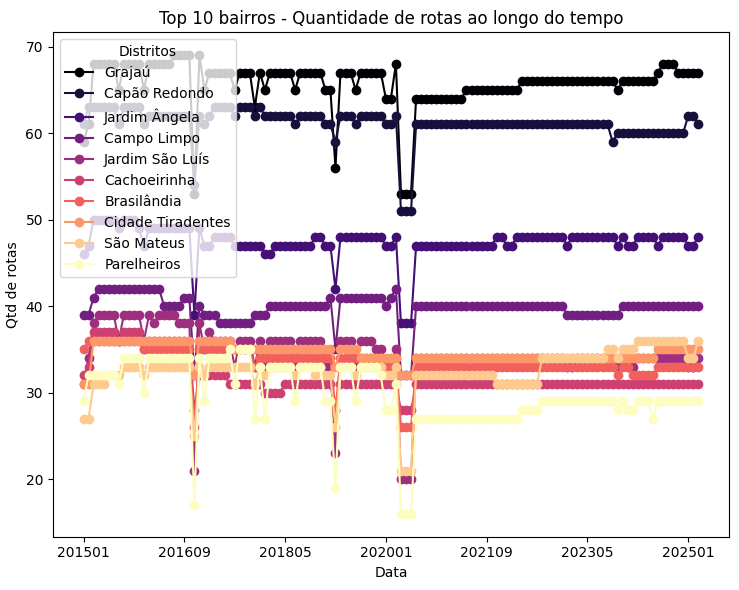
\includegraphics[width=0.75\textwidth]{figuras/rotas e paradas/qtd de rotas e paradas ao longo do tempo por bairro 2.png}
    
    \caption{Histórico da quantidade única de rotas e paradas ao longo do tempo por bairro. Fonte: A própria autora.}
    
\end{figure}

Entre os distritos com mais paradas, destacam-se Grajaú e Itaquera, ficando no topo do ranking ao longo de toda a série histórica. Já entre as rotas, destacam-se Grajaú e Capão Redondo. Apesar de Itaquera possuir muitas paradas, há poucas linhas, indicando que a região é atendida por linhas estruturadas para serem mais longas, possivelmente tendo percursos maiores. No gráfico abaixo, podemos observar que a distância média das rotas que passam em Itaquera é de 27.47 km, enquanto que a média da cidade é de 23.63 km. Essa diferença de quase 4 km ilustra o maior percurso das rotas do bairro.

\begin{figure}[H]
    \centering
    % \subfloat[Média da distância percorrida pelas rotas de Itaquera]
    {%
        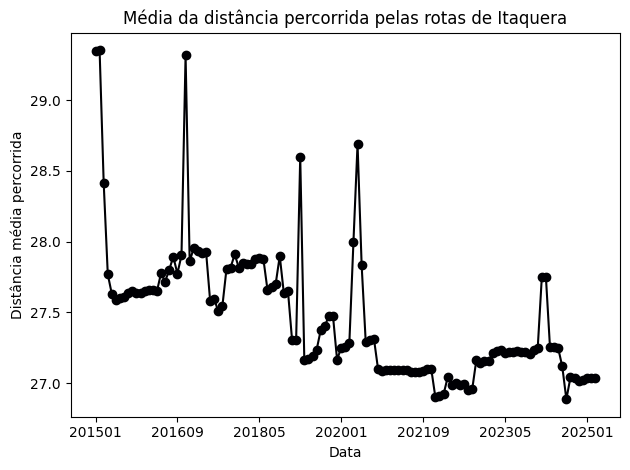
\includegraphics[width=0.75\textwidth]{figuras/rotas e paradas/distancia media percorrida pelas rotas itaquera.png}
    }
    \hspace{0.05\textwidth}
    % \subfloat[Média da distância percorrida pelas rotas da cidade]
    {%
        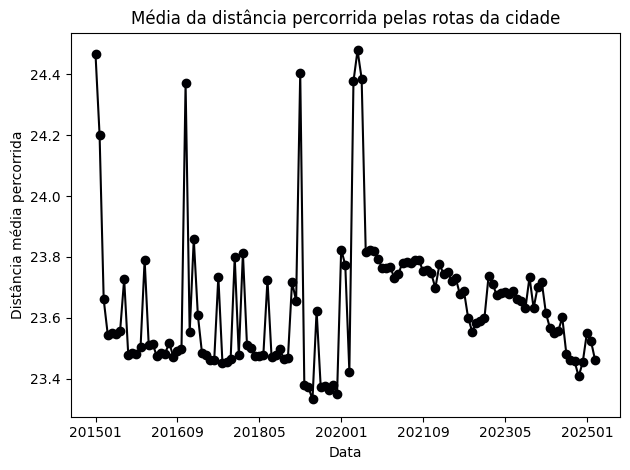
\includegraphics[width=0.75\textwidth]{figuras/rotas e paradas/distancia media percorrida pelas rotas sp.png}
    }
    \caption{Comparação entre a média das distâncias percorridas entre as rotas de Itaquera e as da cidade ao longo do tempo. Fonte: A própria autora. }
    \label{fig:comparacao}
\end{figure}

\subsubsection{Divisão por proximidade a trem e metrô}

Podemos buscar analisar quais estações de metrô ou trem possuem os maiores números de rotas próximas, para entender a importância da integração desses transportes e os possíveis impactos de novas estações.

\begin{figure}[H]
    \centering
    {%
        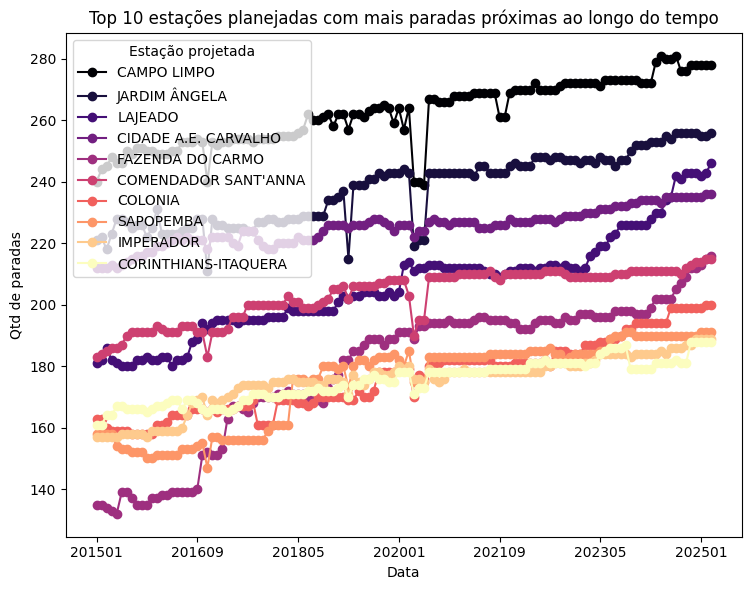
\includegraphics[width=0.75\textwidth]{figuras/rotas e paradas/rotas e paradas ao longo do tempo por estações planejadas 1.png}
    
    \vspace{0.5cm}
    
    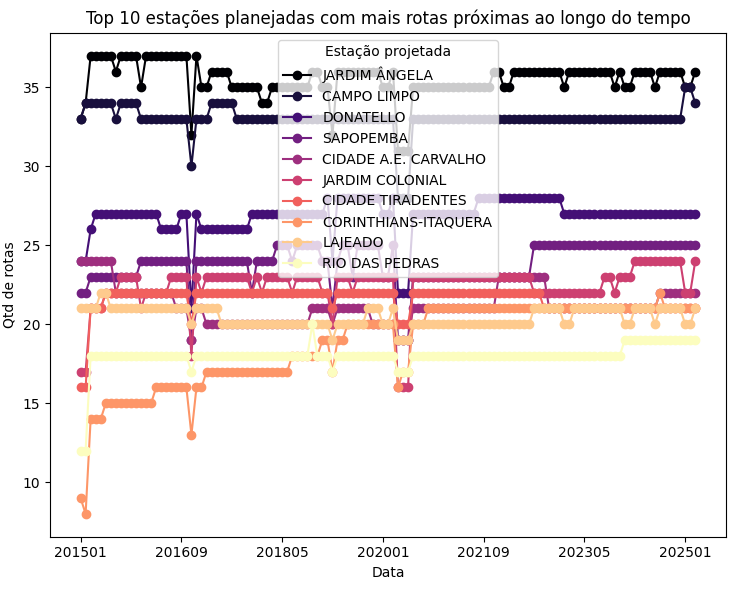
\includegraphics[width=0.75\textwidth]{figuras/rotas e paradas/rotas e paradas ao longo do tempo por estações planejadas 2.png}
    
    }
    \caption{Histórico da quantidade única de rotas e paradas ao longo do tempo por estação mais próxima nas estações futuras. Fonte: A própria autora. }
    
\end{figure}

Entre as estações planejadas, Campo Limpo e Jardim Ângela se destacam por apresentarem o maior número de paradas e rotas próximas, mantendo-se no topo do ranking ao longo de toda a série histórica. A estação Campo Limpo já existe na Linha Lilás, mas também há planos de construir uma integração com a futura linha ALPHAVILLE - CAMPO LIMPO. Já o Jardim Ângela conta com uma ampla rede de transporte, possuindo um terminal de ônibus, e se beneficiaria muito de uma nova estação de metrô que encurtasse o percurso da população, afinal, apesar de ser mais caro que os ônibus, o metrô é mais rápido e eficiente ao transportar passageiros.

\begin{figure}[H]
    \centering
    {%
        

          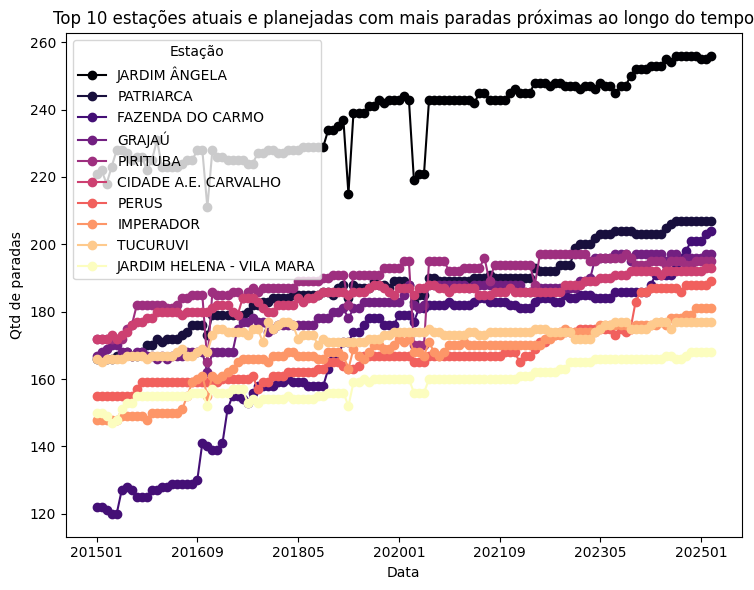
\includegraphics[width=0.75\textwidth]{figuras/rotas e paradas/rotas e paradas ao longo do tempo por estações atuais e planejadas 1.png}
    
    \vspace{0.5cm}
    
    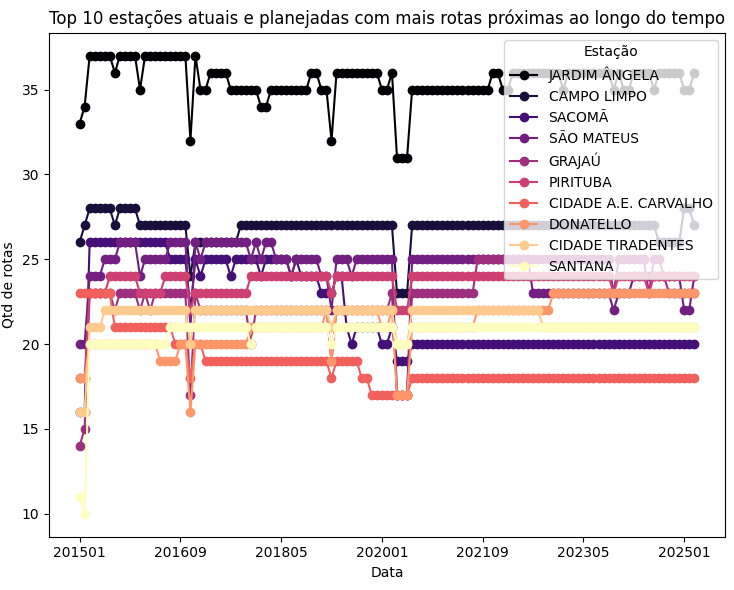
\includegraphics[width=0.75\textwidth]{figuras/rotas e paradas/rotas e paradas ao longo do tempo por estações atuais e planejadas 2.png}
        
    }
    \caption{Histórico da quantidade única de rotas e paradas ao longo do tempo por estação mais próxima nas estações futuras e atuais. Fonte: A própria autora. }
    
\end{figure}

Quando observamos o ranking utilizando dados tanto das estações existentes quanto das futuras, podemos ver que o Jardim Ângela segue sendo o líder em quantidade de rotas e paradas, ou seja, é uma região que se beneficiaria muito da construção da estação. Segundo o \citet{previsao_jd_angela}, a estação Jardim Ângela da Linha Lilás tem início de operação planejado para 2028. 

De acordo com a \citet{previsao_jd_angela_agenciamural}, "Atualmente, o trecho entre o Jardim Ângela até a estação Santa Cruz leva, em média, 1h15 para ser percorrido de ônibus e metrô. Segundo estudo realizado pela Via Mobilidade, após a conclusão das obras, os passageiros levarão cerca de 33 minutos entre o Jardim Ângela e a estação Chácara Klabin." Considerando que a estação Santa Cruz é uma antes da Chácara Klabin, podemos considerar que o percurso do Jardim Ângela até a Santa Cruz levaria cerca de 30 minutos de metrô, uma otimização de 46\%.

Como podemos ver no boxplot abaixo, as rotas que do distrito Jardim Ângela possuem uma alta quantidade de passageiros, com muitos outliers acima de 600 mil passageiros por mês. O Jardim Ângela possui uma das linhas que transporta mais passageiros mensalmente, fato que abordaremos mais para frente na seção de rankings. A matéria prevê que um pico de 62 mil pessoas utilizem a estação por dia, sendo que a região possui mais de 311 mil moradores, segundo o censo de 2022.

\begin{figure}[H]
    \centering
    {%
        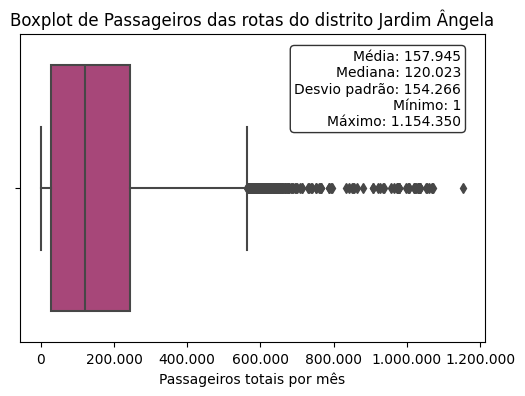
\includegraphics[width=0.6\textwidth]{figuras/rotas e paradas/boxplot_jd_angela.png}
    }
    \caption{Boxplot da quantidade de passageiros nas rotas que passam no distrito Jardim Ângela. Fonte: A própria autora. }
    
\end{figure}

\subsection{Novas linhas e paradas ao longo do tempo}

Como temos o histórico de 10 anos de paradas e rotas, podemos criar uma base que nos diga quantas paradas e rotas novas surgiram em dado mês, utilizando dados do mês anterior. Com exceção de janeiro de 2015, podemos fazer isso para todos os meses subsequentes, até março de 2025. 

No gráfico abaixo, é possível ver que a quantidade de paradas e rotas novas aumentou quase constantemente ao longo do tempo, com exceções em alguns meses, onde possivelmente houve uma reestruturação. Vale notar que a quantidade de meses em que a quantidade de rotas excedeu o padrão quase constante é muito maior que os meses em que a quantidade de paradas excedeu o padrão quase constante. Uma possível explicação para isso é assumir que rotas são mais propensas a serem reestruturadas e criadas do que paradas, já que as rotas dependem das paradas, ou seja, é mais fácil criar uma rota nova que atenda paradas já existentes e algumas paradas novas, do que criar uma parada nova e tentar encaixar ela em rotas já existentes.

\begin{figure}[H]
    \centering
    {%
        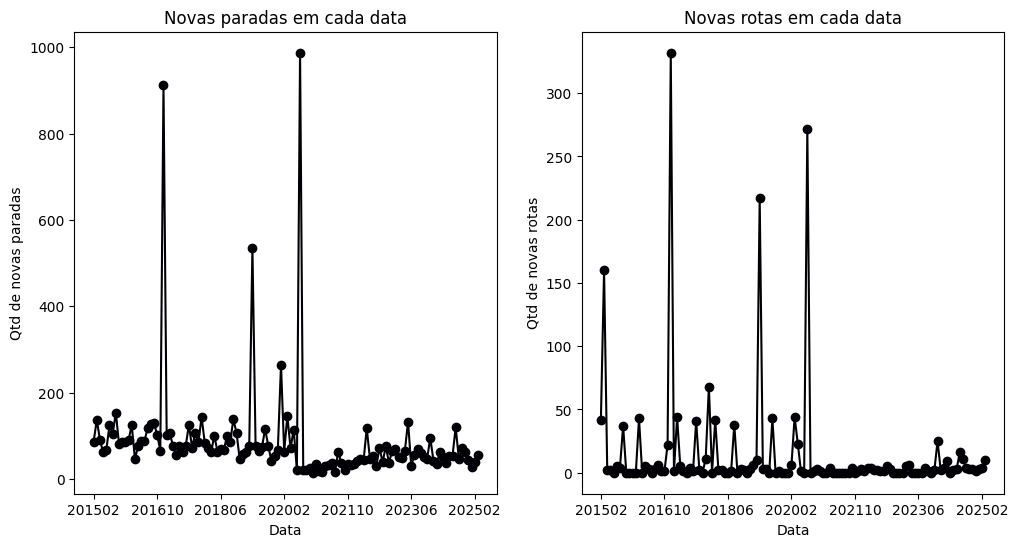
\includegraphics[width=1\textwidth]{figuras/rotas e paradas/Novas parada e rotas por data.png}
    }
    \caption{Quantidade de novas paradas e rotas ao longo do tempo. Fonte: A própria autora.}
    
\end{figure}

Para essa métrica, também podemos analisar o gráfico discriminado por região (zona), bairro (distrito) e estação próxima. Para as estações, consideraremos apenas as que já existem, já que não faz tanto sentido considerar que ocorreu um replanejamento do sistema de transporte para estações que não existem ainda.

\subsubsection{Divisão por região}


\begin{figure}[H]
    \centering
    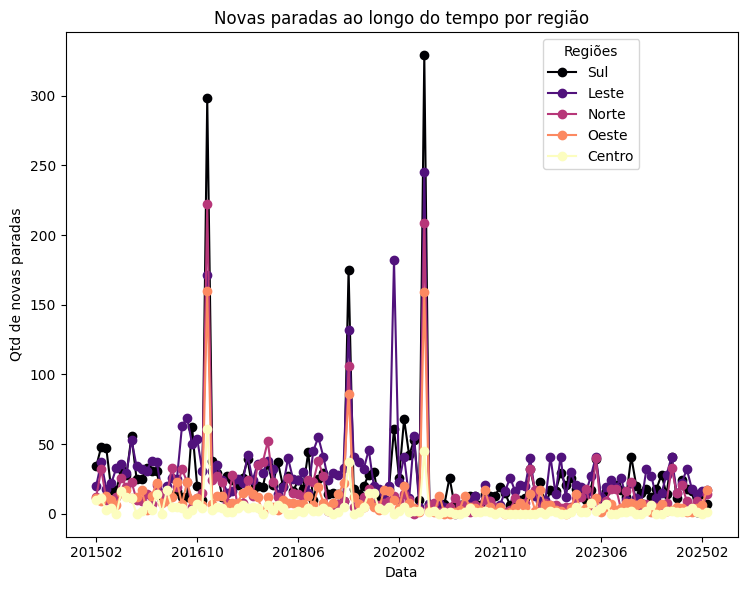
\includegraphics[width=0.75\textwidth]{figuras/rotas e paradas/Novas parada por data e zona.png}
    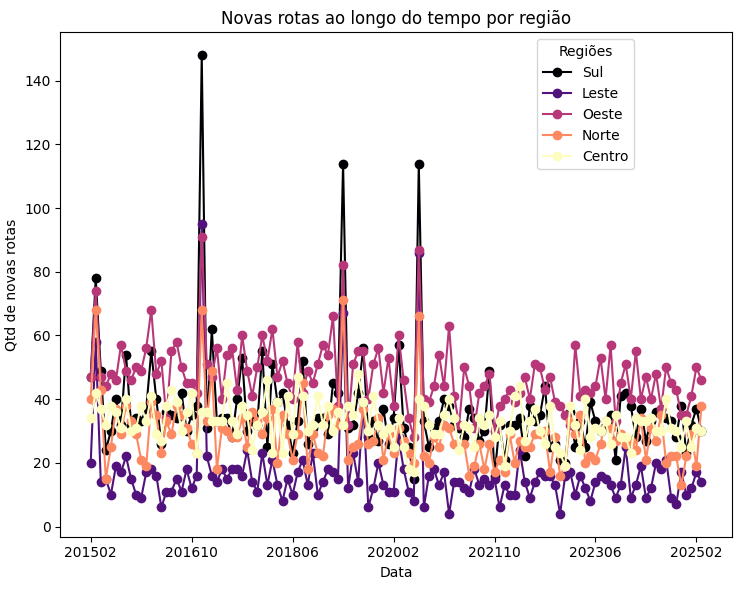
\includegraphics[width=0.75\textwidth]{figuras/rotas e paradas/Novas rotas por data e zona.png}\\
    \caption{Quantidade de novas paradas e rotas ao longo do tempo por região. Fonte: A própria autora}
\end{figure}

Pela primeira vez, vemos que a Zona Oeste e o Centro se destacam. Ambas apresentam uma maior quantidade de rotas novas ao longo do tempo, sem necessariamente ter um aumento no número de paradas, o que pode significar que essas duas regiões receberam uma maior atenção do planejamento de transporte. Vimos anteriormente que as zonas Leste e Sul possuem um alto número de rotas e paradas totais, mas vemos aqui que elas não possuem tanto destaque no número de novas rotas e paradas.

\subsubsection{Divisão por bairro}
\begin{figure}[H]
    \centering
     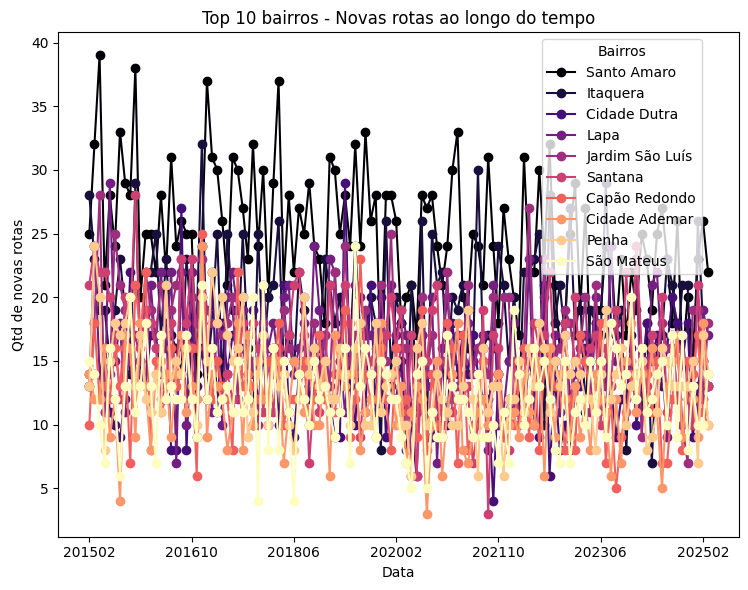
\includegraphics[width=0.75\textwidth]{figuras/rotas e paradas/Novas rotas por data e bairro.png}
    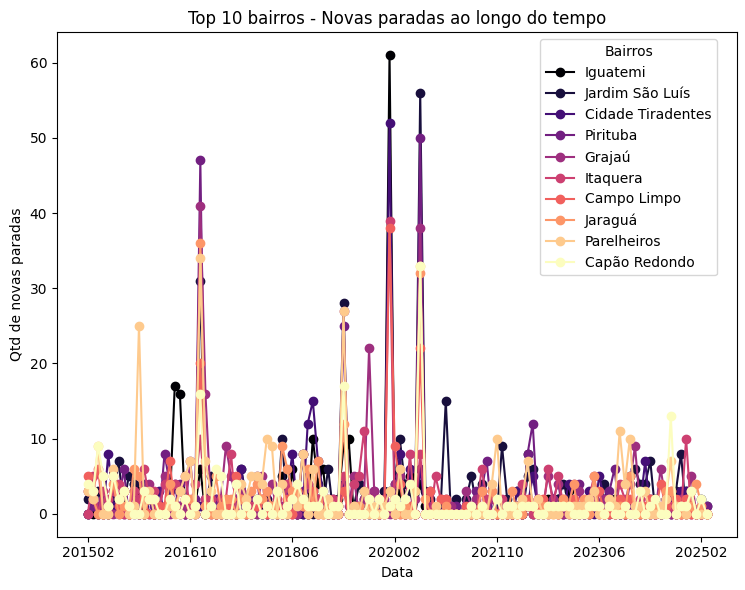
\includegraphics[width=0.75\textwidth]{figuras/rotas e paradas/Novas parada por data e bairro.png}\\
    \caption{Quantidade de novas paradas e rotas ao longo do tempo por bairro. Fonte: A própria autora}
    
\end{figure}

Nos gráficos por bairro, notamos uma dominância de Santo Amaro e Itaquera nas novas rotas, demonstrando que as duas regiões foram alvos de um recente planejamento mais intensivo do transporte. 

\subsubsection{Divisão por estação mais próxima}
\begin{figure}[H]
    \centering
     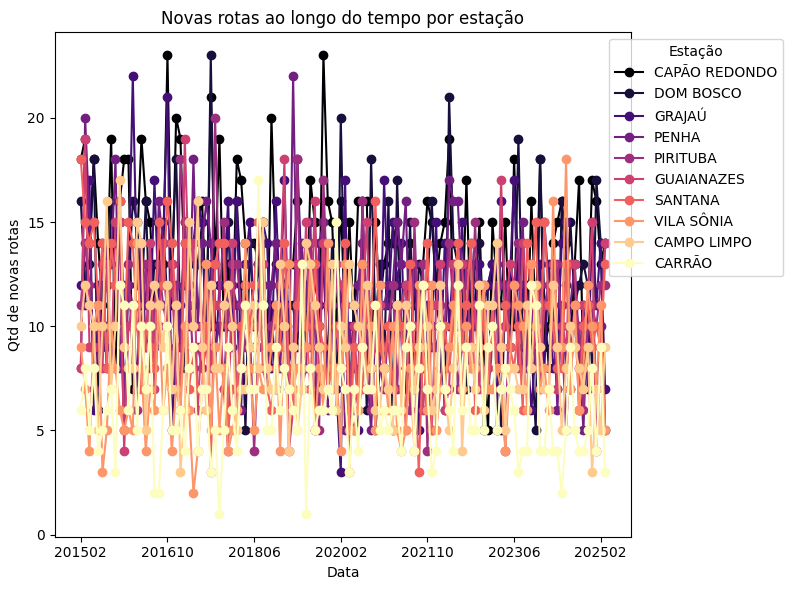
\includegraphics[width=0.75\textwidth]{figuras/rotas e paradas/Novas rotas por data e estacao.png}
    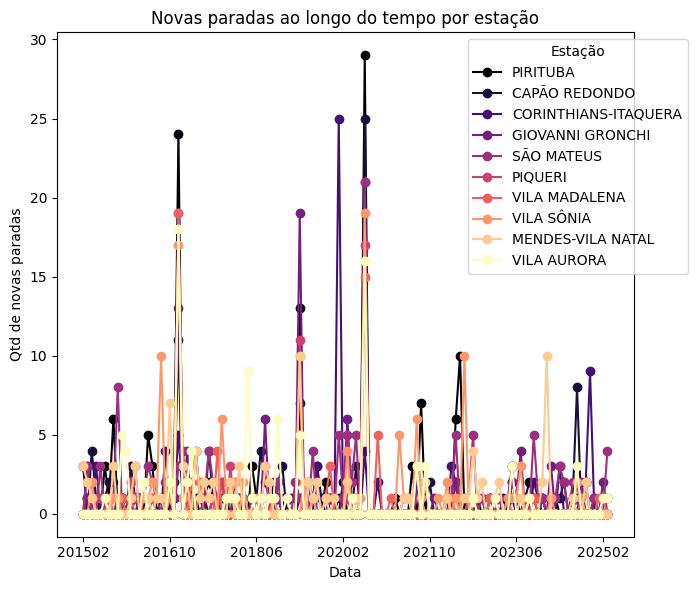
\includegraphics[width=0.75\textwidth]{figuras/rotas e paradas/Novas parada por data e estacao.png}\\
    \caption{Quantidade de novas paradas e rotas ao longo do tempo por estação mais próxima (considerando apenas as existentes). Fonte: A própria autora }
    
\end{figure}

Por fim, ao analisar os gráficos de novas rotas próximo a estações, notamos uma leve dominância da estação Capão Redondo. Em especial, em 2018, houve mais de 25 linhas novas próximas a estação. Podemos levantar a hipótese de uma reestruturação após a concessão para a ViaMobilidade, que ocorreu no mesmo período, mas não encontramos nada que prove essa hipótese.

\subsection{Correlação com a população}

Mês a mês, podemos calcular quantas pessoas moram no subdistrito ao qual uma parada pertence. Como a cidade de São Paulo é muito fragmentada, o número de subdistritos é alto. A partir desses dados, podemos analisar a correlação entre a quantidade total de rotas ou paradas, e a soma da população imediatamente relacionada a elas.

A principio, podemos supor que, quanto maior o número de paradas, maior a quantidade de pessoas afetadas por essas paradas. Caso essa relação linear positiva não exista, vamos concluir que o sistema de transporte está criando paradas não eficientes, muito próximas, que atendem ao mesmo número de pessoas, ou seja, concentrando as paradas em um único local, ao invés de expandir o alcance do transporte para afetar mais pessoas. Desse modo, para testar essa hipótese, elaboramos o gráfico abaixo:

\begin{figure}[H]
    \centering
    {%
        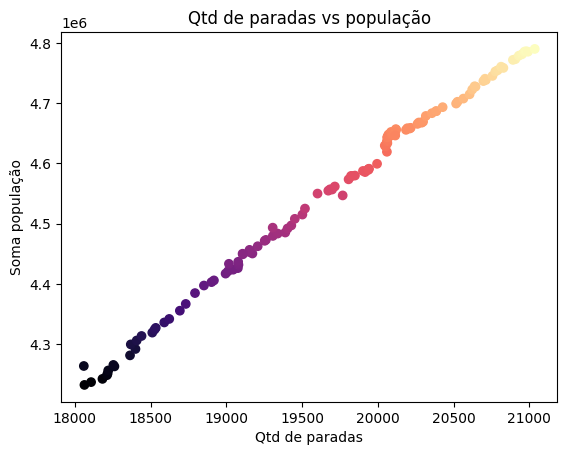
\includegraphics[width=0.7\textwidth]{figuras/rotas e paradas/correlação população e paradas.png}
    }
    \caption{Correlação entre a quantidade de paradas e a quantidade de população imediatamente afetada. Fonte: A própria autora }
    
\end{figure}

Através do gráfico, podemos concluir que quanto maior o número de paradas, maior população afetada, implicando que o sistema está se expandindo de forma eficiente, criando paradas novas em locais onde não havia paradas anteriormente.

Podemos fazer a mesma hipótese para a relação entre quantidade de rotas e população afetada:

\begin{figure}[H]
    \centering
    {%
        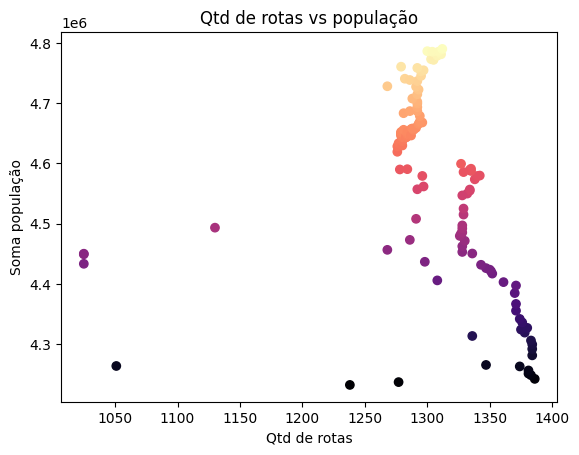
\includegraphics[width=0.7\textwidth]{figuras/rotas e paradas/correlação população e rotas.png}
    }
    \caption{Correlação entre a quantidade de rotas e a quantidade de população imediatamente afetada. Fonte: A própria autora }
    
\end{figure}

No gráfico acima, podemos observar que o número de pessoas diretamente afetadas pelas rotas não está diretamente relacionado com o número de rotas, o que pode nos dizer que há uma possível desigualdade na distribuição do transporte em relação à densidade populacional, ou seja, não devem surgir rotas que façam caminhos totalmente novos, atingindo mais pessoas, mas sim reestruturações de rotas para cobrir áreas que já eram cobertas por outras rotas, mostrando que o sistema pode se tornar mais fragmentado.

\subsection{Análise geral das rotas}

Podemos analisar a distribuição de rotas discriminada por categorias como qual a cor da rota, se ela é noturna, se ela é circular, quantas horas ela opera, se ela atua em dias úteis, todos os dias ou apenas no final de semana e, por fim, uma nuvem de palavras para analisar os nomes mais frequentes nas rotas.

\subsubsection{Rotas por cor}

A SPTrans dividiu a cidade de São Paulo em 8 áreas, e atribuiu uma cor para cada uma, conforme a imagem abaixo. Cada ônibus, portanto, segue essa padronização para a identidade visual externa.

\begin{figure}[H]
    \centering
    {%
        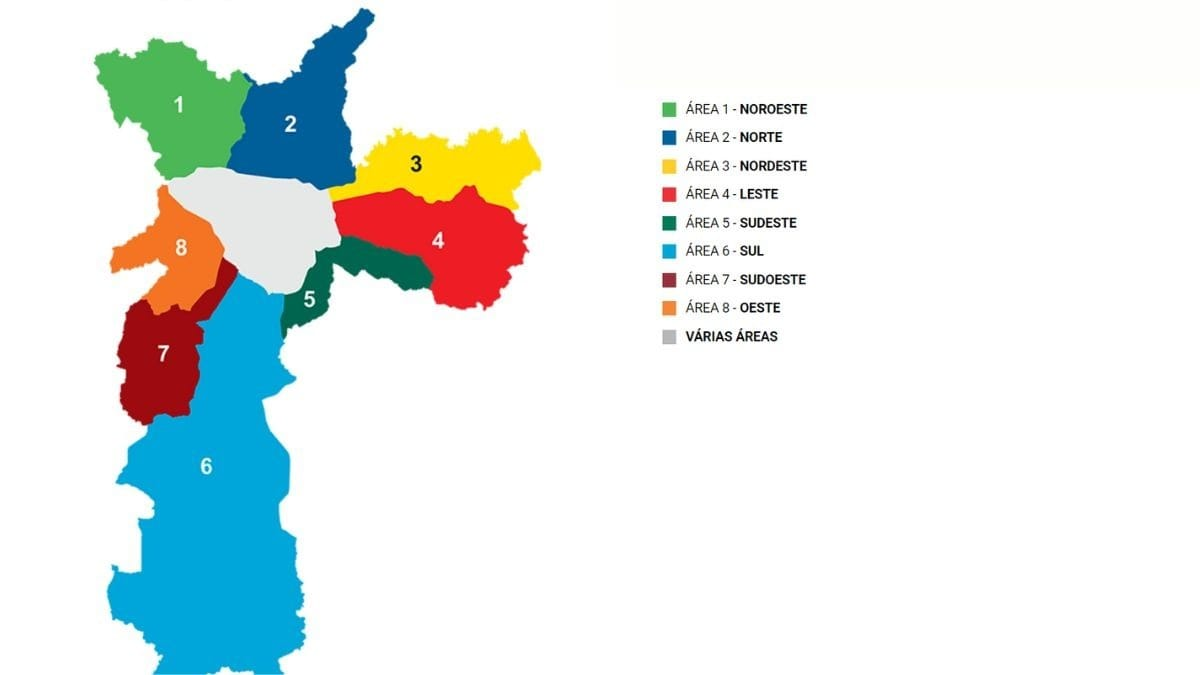
\includegraphics[width=0.85\textwidth]{figuras/mapa-da-divisao-de-cores-dos-onibus-de-sao-paulo-184838.jpg}
    }
    \caption{Mapa da divisão da cidade por cores. Fonte: Band Jornalismo }
    
\end{figure}

Quando analisamos a distribuição das rotas por cor, vemos que ela é praticamente uniforme pela cidade, com uma leve dominância das rotas azul claro (Sul), vinho (Sudoeste) e amarelo (Nordeste).

\begin{figure}[H]
    \centering
    {%
        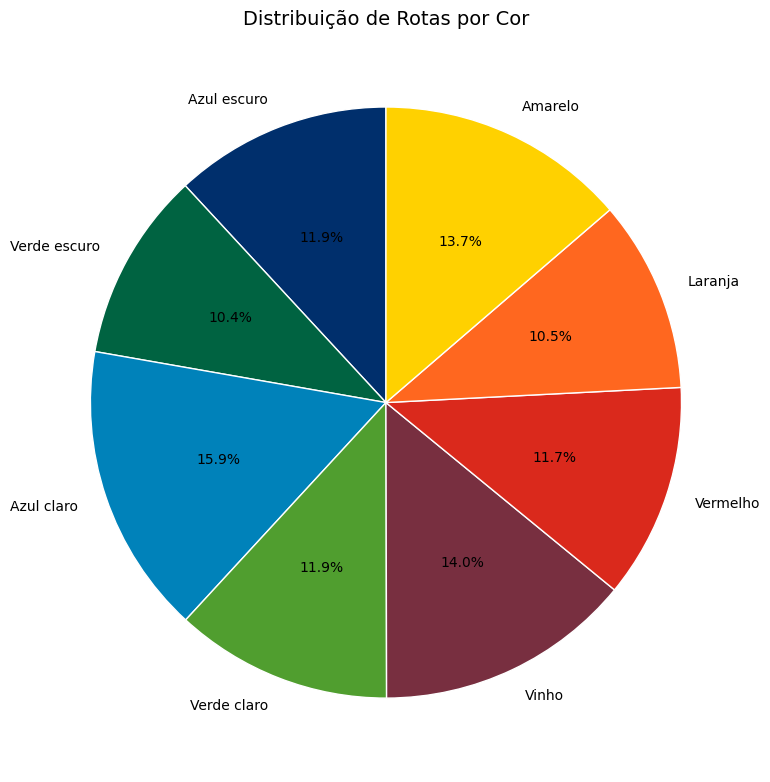
\includegraphics[width=0.75\textwidth]{figuras/rotas e paradas/qtd de rotas por cor.png}
    }
    \caption{Gráfico de pizza da quantidade de rotas por cor da rota. Fonte: A própria autora. }
    
\end{figure}

\subsubsection{Rotas noturnas}

Podemos listar quantas rotas são ou não noturnas. Atribuiremos que uma rota é noturna caso ela opere entre 02h e 03h da manhã.

\begin{table}[H]
\centering
\begin{tabular}{rrr}
\toprule
Tipo & Qtd de rotas & Porcentagem \\
\midrule
Não noturna & 1168 & 74\% \\
Noturna & 411 & 26\% \\
\bottomrule
\end{tabular}
\caption{Quantidade de rotas noturnas. Fonte: A própria autora.}
\label{tab:distancias_rotas}
\end{table}

De forma inesperada, 26\% das rotas têm horário de operação noturno. Para essas rotas, vamos analisar qual a distribuição dos horários de operação, para verificar se há muitas rotas que são apenas noturnas (operam poucas horas no dia), ou se essa porcentagem foi inflada por rotas que operam no período diurno e noturno:


\begin{figure}[H]
    \centering
    {%
        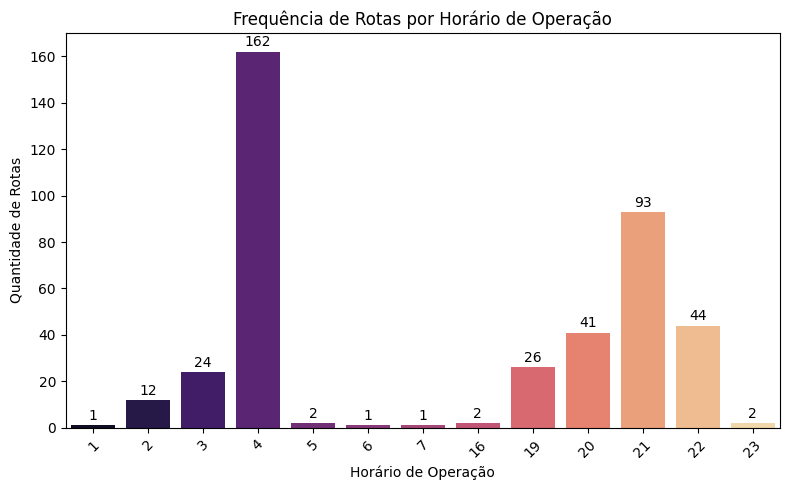
\includegraphics[width=0.8\textwidth]{figuras/rotas e paradas/freq das rotas noturnas por horario.png}
    }
    \caption{Horário de operação das rotas noturnas. Fonte: A própria autora. }
    
\end{figure}

Como podemos ver no gráfico acima, muitas das rotas noturnas operam apenas no horário noturno, entretanto, temos que cerca de 50\% das rotas consideradas noturnas operam mais que 19 horas por dia. Logo, nossa suspeita inicial estava correta, e realmente há muitas rotas que não são apenas noturnas na contagem das rotas noturnas, o que explica por que temos cerca de 25\% das rotas da cidade consideradas noturnas.

\subsubsection{Rotas circulares}

Podemos listar quantas rotas são ou não circulares. Atribuimos que uma rota é circular caso ela tenha apenas uma direção na base de viagens.

\begin{table}[H]
\centering
\begin{tabular}{lr}
\toprule
Direção & Qtd de rotas \\
\midrule
Circular & 497 \\
Não circular & 1082 \\
\bottomrule
\end{tabular}
\caption{Quantidade de rotas por direção. Fonte: A própria autora.}
\label{tab:qtd_rotas_direcao}
\end{table}

A maioria das rotas é não circular. Uma possível hipótese é que as rotas circulares percorrem distâncias menores do que as não circulares, uma vez que seu objetivo pode ser a conexão de pontos dentro de um mesmo bairro, e não a ligação entre diferentes regiões da cidade.

\begin{figure}[H]
    \centering
    {%
        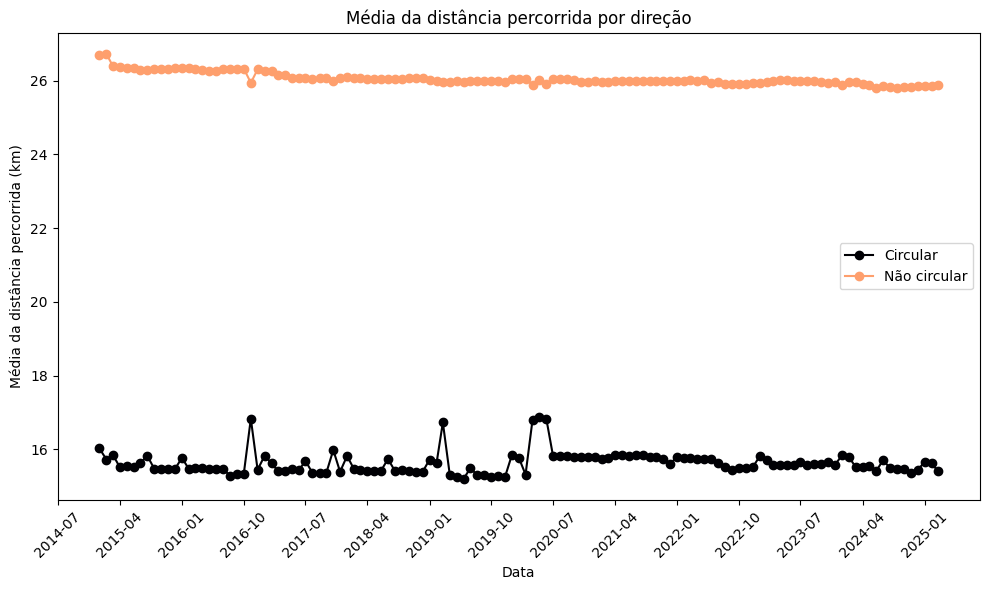
\includegraphics[width=0.9\textwidth]{figuras/rotas e paradas/media dist percorrida rotas circulares.png}
    }
    \caption{Média da distância percorrida por rotas, sendo elas circulares ou não. Fonte: A própria autora. }
    
\end{figure}

\vspace{-1cm}

Logo, concluímos que a maioria das rotas da cidade é não circular, e a média das distâncias que as circulares percorrem é cerca de 10 km menor que a média das não circulares.

\subsubsection{Frequência de operação}

Utilizando todos os dados históricos do GTFS, podemos avaliar qual a distribuição das frequências de operação das rotas ao longo do dia.

\begin{figure}[H]
    \centering
    {%
        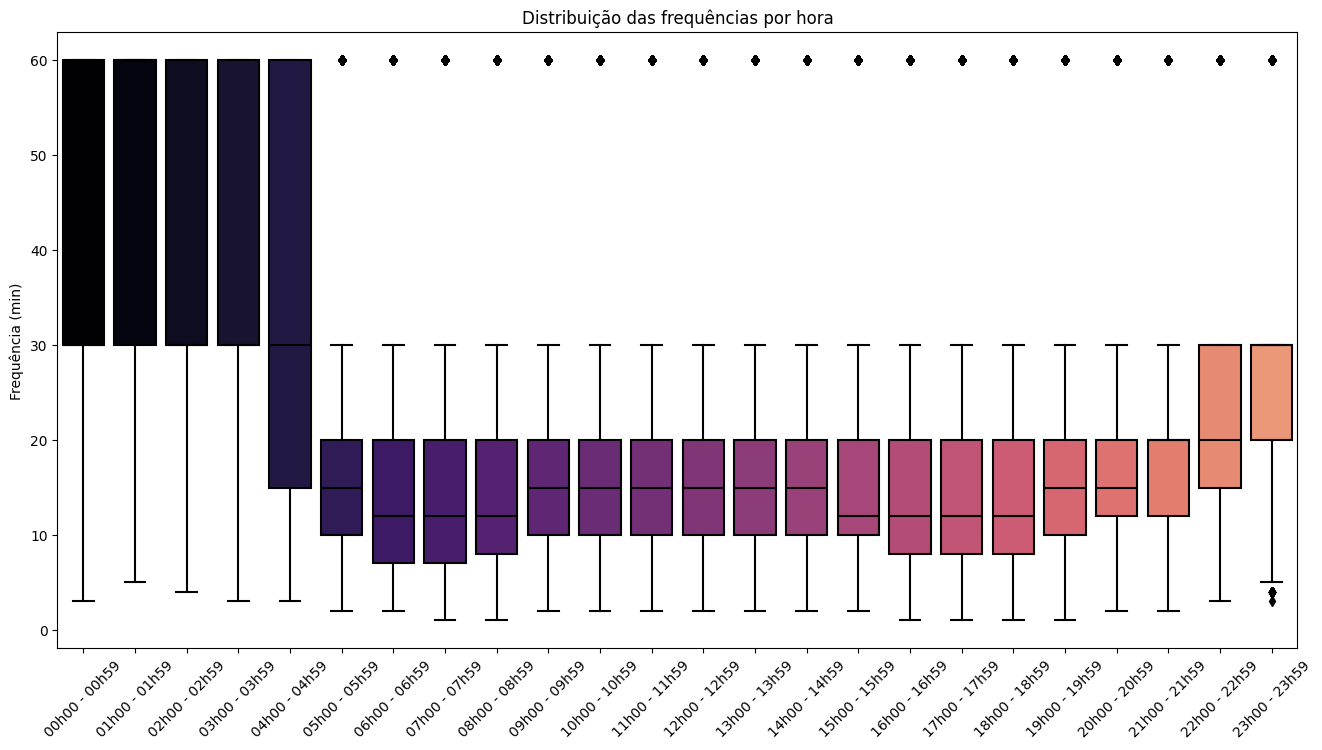
\includegraphics[width=0.9\textwidth]{figuras/rotas e paradas/boxplot frequencias.png}
    }
    \caption{Boxplot da frequência de operação das linhas por horário considerando todo o histórico do GTFS. Fonte: A própria autora. }
    
\end{figure}

\vspace{-2cm}

Podemos notar que, durante a noite, a maioria das rotas opera com frequência entre 30 minutos e 1 hora. Entre 04h e 23h59, temos algumas linhas outliers, que operam a cada 60 minutos, e a maioria ficando, na mediana, entre 10 e 20 minutos. Além disso, a variabilidade em algumas horas é grande, indicando que algumas rotas funcionam muito diferente das outras no mesmo horário.

Esses dados são surpreendentes pois a impressão que temos é de que as linhas operam com frequências muito maiores do que o mostrado no gráfico. Vale lembrar que horários programados são diferentes dos horários reais das linhas, que podem sofrer alterações devido ao trânsito e serem replanejadas ao longo do dia. Também é comum que o ônibus de um horário se atrase, e acabe passando junto com o ônibus do próximo horário.

Vamos elaborar o mesmo boxplot para as rotas que circulam na região Oeste, em particular, as que circulam na subprefeitura do Butantã, para buscar entender se essas estatísticas mudam conforme os locais que consideramos.

\begin{figure}[H]
    \centering
    {%
        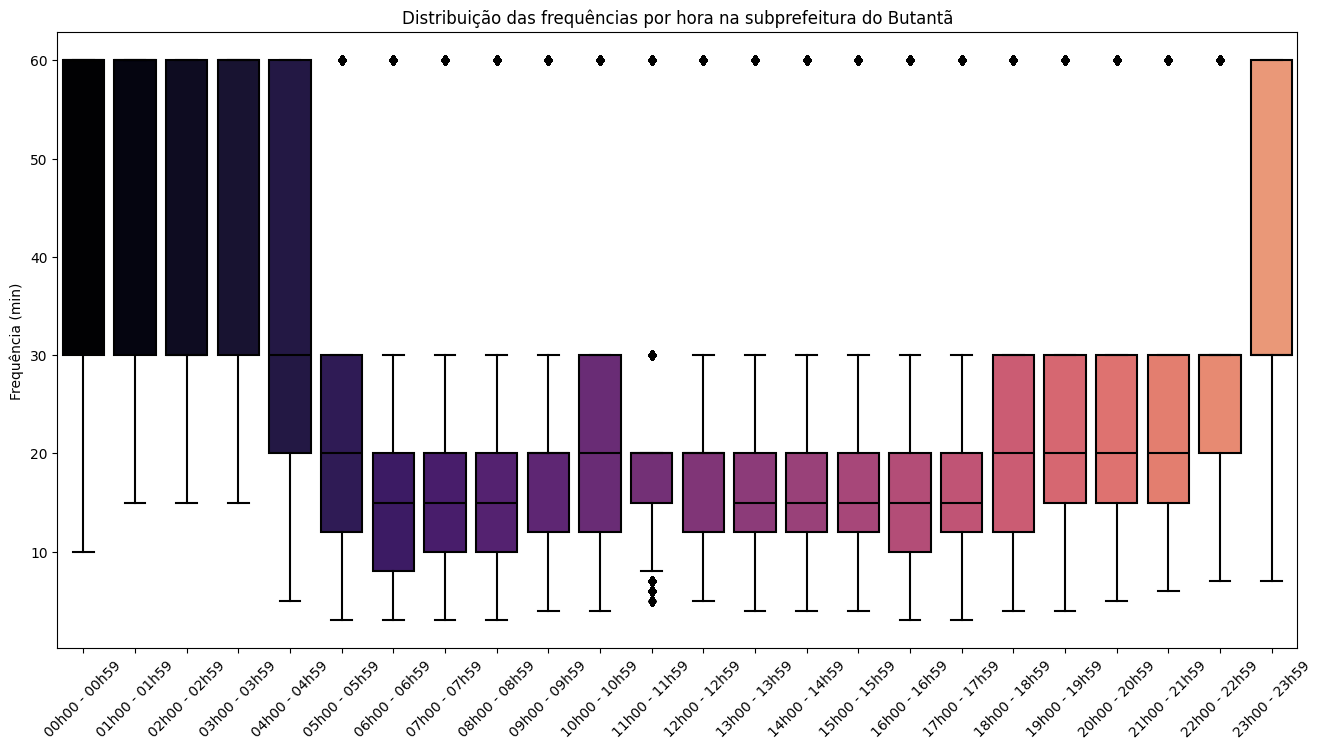
\includegraphics[width=0.9\textwidth]{figuras/rotas e paradas/boxplot frequencias butanta.png}
    }
    \caption{Boxplot da frequência de operação das linhas da subprefeitura do Butantã por horário. Fonte: A própria autora. }
    
\end{figure}


Podemos observar que a distribuição das frequências é diferente nas rotas que passam no Butantã. Essa diferença é mais perceptível em horários de pico, como entre 09h e 09h59 e entre 18h e 18h59, período em que as rotas do Butantã operam mais lentamente do que as rotas de toda a cidade.


\subsubsection{Dias de operação}

Vamos analisar qual a distribuição das rotas por dia de operação. Imaginamos que a maioria das rotas opere todos os dias.

\begin{figure}[H]
    \centering
    {%
        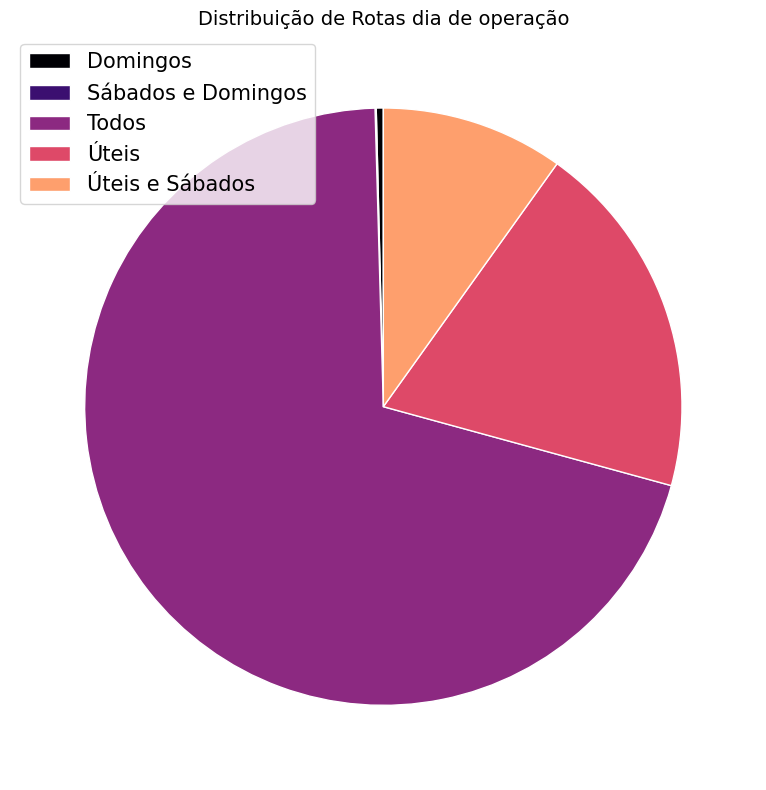
\includegraphics[width=0.5\textwidth]{figuras/rotas e paradas/distribuição das rotas por dias de operacao.png}
    }
    \caption{Gráfico de pizza dos dias de operação das rotas considerando todo o histórico do GTFS. Fonte: A própria autora. }
    
\end{figure}

Como podemos observar no gráfico, a maioria das rotas opera todos os dias, seguido pelas rotas que operam apenas nos dias úteis e as que operam apenas em dias úteis e sábados. Vale notar que pouquíssimas rotas operam exclusivamente no final de semana, a ponto de não serem visíveis no gráfico.

\subsubsection{Nome das rotas}

Uma das maneiras de visualizar quais os nomes mais frequentes nas rotas é com uma nuvem de palavras. Para a elaboração da nuvem, retiramos dos nomes das rotas palavras como "jardim", "vila", "terminal", "são", "metrô" e etc, pois o intuito da análise é observar os locais que aparecem mais frequentemente nos nomes. Além disso, consideramos aqui rotas únicas, sendo que uma rota só vai aparecer duas vezes na base utilizada para gerar as visualizações caso tenha mudado de nome ao longo dos 10 anos de dados. 

\begin{figure}[H]
    \centering
    {%
        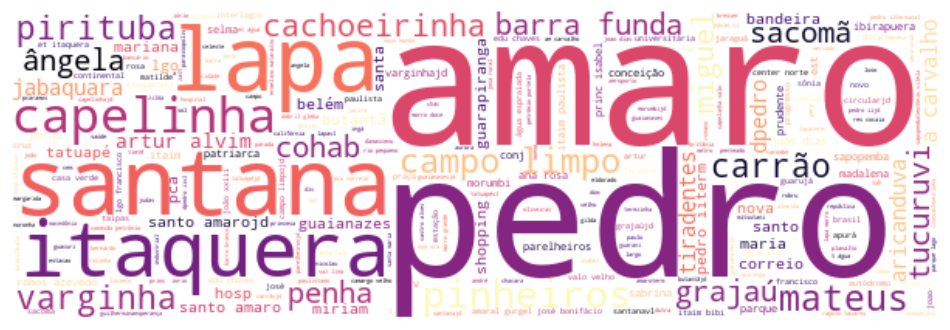
\includegraphics[width=0.8\textwidth]{figuras/rotas e paradas/wordcloud.png}
    }
    \caption{Nuvem de palavras com os nomes das rotas. Fonte: A própria autora. }
    
\end{figure}

 Podemos notar uma dominância de locais onde há terminais, como Terminal Pinheiros, Terminal Pq D. Pedro II, Terminal Santana, Terminal Lapa e etc. Vale notar que a palavra "Cohab" apareceu na nuvem, com 42 menções no total, destacando a importância do projeto social na cidade. Na tabela abaixo podemos as top 20 palavras mais frequentes nos nomes:


\begin{longtable}{lr}
\caption{Frequência das palavras nos nomes das rotas. Fonte: A própria autora.}
\label{tab:distancias_rotas} \\

\toprule
Palavra & Frequência \\
\midrule
\endfirsthead

\multicolumn{2}{c}{\tablename\ \thetable{} -- continuação} \\
\toprule
Palavra & Frequência \\
\midrule
\endhead

\midrule
\multicolumn{2}{r}{\textit{continua}} \\
\endfoot

\bottomrule
\endlastfoot

pedro & 142 \\
amaro & 132 \\
santana & 101 \\
lapa & 101 \\
itaquera & 88 \\
santo & 87 \\
capelinha & 80 \\
campo & 79 \\
pinheiros & 69 \\
pirituba & 67 \\
limpo & 66 \\
mateus & 66 \\
barra & 57 \\
varginha & 53 \\
carrão & 52 \\
itaim & 50 \\
cachoeirinha & 50 \\
sacomã & 47 \\
joão & 46 \\
maria & 45 \\

\end{longtable}

\subsection{Ranking de rotas}

Podemos rankear as rotas com diversas variáveis: nessa seção, vamos elaborar visualizações para analisar quais rotas possuem mais passageiros e maior distância percorrida. Não vamos analisar o ranking das linhas que tem menos passageiros ou menor distância percorrida pois, ao analisar a base, notamos que não há um ranking claro, devido a inconsistências como rotas que operaram por pouco tempo ou que possuem dados faltantes.

\subsubsection{Ranking de rotas por passageiros}

Para tornar a comparação mais justa com as rotas que foram surgindo ao longo dos anos, vamos criar o ranking com base na média mensal de passageiros, utilizando o total de passageiros que pegaram uma rota.

\begin{table}[H]
\centering
\begin{tabular}{lr}
\toprule
Linha & Qtd de passageiros \\
\midrule
431010 - E.T.ITAQUERA/TERM PQ D PEDRO   & 768.837 \\
675K10 - TERM JD ANGELA-METRO STA CRUZ & 730.417 \\
220210 - HOSP ITAIM/GUAIAZAZES & 691478 \\
691310 - TERM BANDEIRA/TERM VARGINHA & 667.461 \\
607C10 - JD MIRIAM/SHOPP MORUMBI & 651849 \\
870010 - T CAMPO LIMPO/PCA R D AZEVEDO  & 619.228 \\
600010 - TERM PARELHEIROS/TERM SANTO AM & 617.841 \\
431310 - T CID TIRADENTES/T PQ D PEDRO  & 610.069 \\
978T10 - JD GUARANI/METRO BARRA FUNDA & 585.280 \\
376310 - TERM VL CARRAO/METRO TATUAPE & 574.801 \\
\bottomrule
\end{tabular}
\caption{Ranking das top 10 linhas com mais passageiros mensalmente em média. Fonte: A própria autora.}
\label{tab:distancias_rotas}
\end{table}

Creio que não seja surpresa, ao menos para moradores de São Paulo, que as linhas mais movimentadas estão em regiões como Itaquera, Jd. Ângela, Guaianazes, Campo Limpo, Parelheiros, Cidade Tiradentes e etc, pois são regiões superpopuladas. Vale notar que todas as linhas no ranking fazem o transporte de um bairro para o centro ou o metrô, ou seja, são linhas necessárias para transportar os moradores de seus bairros até o trabalho.

\subsubsection{Ranking de rotas por distância percorrida}

Para saber quais são as rotas que percorrem as maiores distâncias na cidade, vamos utilizar a distância percorrida pelo dado mais recente da rota. Então, por exemplo, se uma rota existiu entre 2015 e 2018, vamos utilizar o dado de distância percorrida por ela no último mês de 2018 em que ela existiu. Assim, conseguimos contemplar os dados mais recentes de cada rota, sem deixar de fora as rotas que foram reestruturadas ao longo de 10 anos de base.

\begin{table}[H]
\resizebox{\textwidth}{!}{%
\centering
\begin{tabular}{llr}
\toprule
Id da rota & Nome da rota & Distância percorrida \\
\midrule
331010 & Term. Amaral Gurgel - Cidade Tiradentes (circular) & 90.228783 \\
213C10 &  Vl. Califórnia - Itaim Paulista & 75.915440 \\
477P10 & Ipiranga - Rio Pequeno & 70.842332 \\
695Y10 &  Term. Parelheiros - Metrô Vl. Mariana & 68.280425 \\
400251 & Guaianazes - Pq. D.pedro II & 67.346256 \\
345910 & Itaim Paulista - Term. Pq. D.pedro II & 64.141479 \\
536210 & Pq. Res. Cocaia - Pça. Da Sé & 63.219958 \\
393H10 & Term. Amaral Gurgel - Jd. Sto André & 62.951140 \\
353910 & Cid. Tiradentes - Metrô Bresser & 62.516246 \\
957T10 & Cohab Taipas - Itaim Bibi, Cohab Taipas - Vl. Olímpia & 61.882924 \\
\bottomrule
\end{tabular}
}
\caption{Ranking das top 10 linhas com maior distância percorrida. Fonte: A própria autora.}
\label{tab:distancias_rotas}
\end{table}

A primeira linha, 331010, foi extinta em 2015, por uma reestruturação da SPTrans. Essa linha tinha operação exclusivamente noturna, e era conhecida como "Rainha da Madrugada", operando do centro até a Cidade Tiradentes, e transportando 10 mil passageiros por mês, com frequência de 1h. Vale notar que, pela linha ser circular, a distância é calculada considerando a ida e volta. Ainda, segundo o \citet{rainha_da_madrugada}, a linha possuia 102 km, número que difere em 12 km a distância que calculamos. possivelmente, essa discrepância aparece por diferenças no método de cálculo. 

A segunda linha, 213C10, que ligava a Vila Califórnia ao Itaim Paulista, foi extinta em 2018. Ela atravessava a cidade e não era circular, ou seja, eram 75km na ida e 75km na volta, totalizando 150 km percorridos. 

A terceira linha com maior distância percorrida é a 477P10, que existe até atualmente, e liga o Rio Pequeno ao Ipiranga, passando por pontes importantes como o Museu do Ipiranga, diversas estações de Metrô, a Faria Lima e a Raposo Tavares. Essa linha também não é circular.

\subsection{Análise de centralidade}

A partir dos grafos criados com a biblioteca Peartree, que consideram as rotas que operam entre 06h e 08h (todas as rotas diurnas, com maior fluxo de passageiros), podemos analisar algumas métricas centralidade. Essas métricas foram calculadas mês a mês para cada parada (nó) do grafo, resultando em uma tabela com o identificador único da parada, a data as respectivas métricas de centralidade: Betweenness Centrality, Degree Centrality e Closeness Centrality.

\subsubsection{Análise temporal}

Como nossos dados são discriminados mês a mês, podemos buscar entender como as métricas de centralidade variaram ao longo do tempo. Inicialmente, vamos agrupar por ano, para facilitar a visualização:

\begin{figure}[H]
    \centering
    {%
        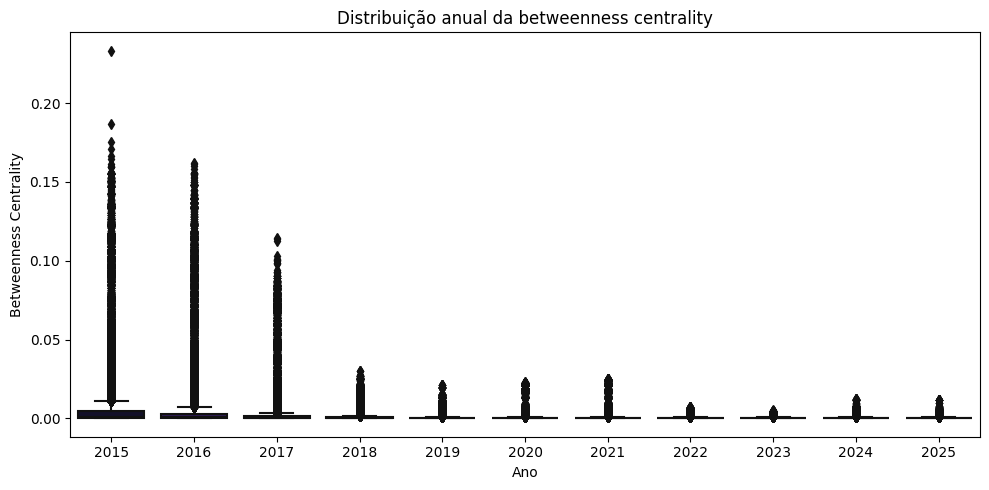
\includegraphics[width=0.85\textwidth]{figuras/centralidade_grafo/betweenness centrality por ano.png}
    }
    \caption{Boxplots da média de betweenness centrality por ano. Fonte: A própria autora. }
    
\end{figure}

Como o betweness centrality retrata o quanto um nó atua como ponte ou intermediário no fluxo da rede, podemos concluir que entre 2015 e 2017, o sistema apresentava valores elevados de betweenness centrality, com alta variância, com uma forte centralização estrutural da rede, em que poucos nós, que desempenhavam papel predominante na conectividade do sistema. A partir de 2018 ocorreu uma redução drástica desses valores, acompanhada de uma diminuição da variabilidade entre os nós, sugerindo que houve uma reestruturação para fragmentar a rede e distribui-la melhor, ou seja, as paradas pararam de ser tão centrais e foram melhor planejadas para conectar a rede, que também se expandiu. Podemos correlacionar isso com a quantidade de paradas existentes no sistema mês a mês: 

\begin{figure}[H]
    \centering
    {%
        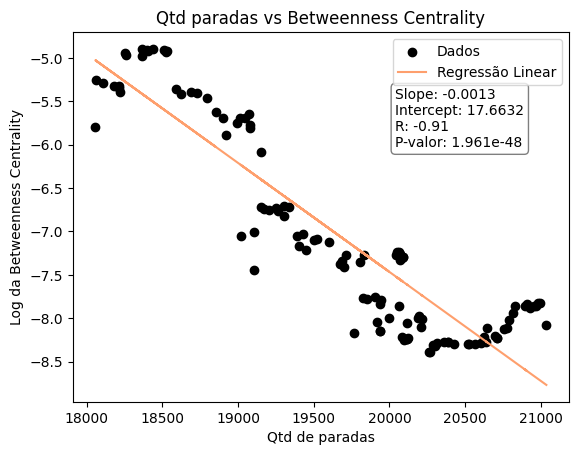
\includegraphics[width=0.55\textwidth]{figuras/centralidade_grafo/correlação betweenness centrality e qtd de paradas.png}
    }
    \caption{Correlação entre o log da média mensal da betweenness centrality e a quantidade mensal de paradas no sistema de transporte. Fonte: A própria autora. }
    
\end{figure}

Podemos concluir, então, que as duas métricas tem uma relação: há uma tendência negativa, quando a rede tem mais paradas, ela fica menos centralizada, com menos dependência de poucos nós críticos. O R=-0,91 e o p-valor=$1,961\times10^{-48}$ nos mostra que a relação é estatisticamente significativa. Através do gráfico abaixo, também podemos observar que os resíduos da regressão se aproximam de uma distribuição normal.

\begin{figure}[H]
    \centering
    {%
        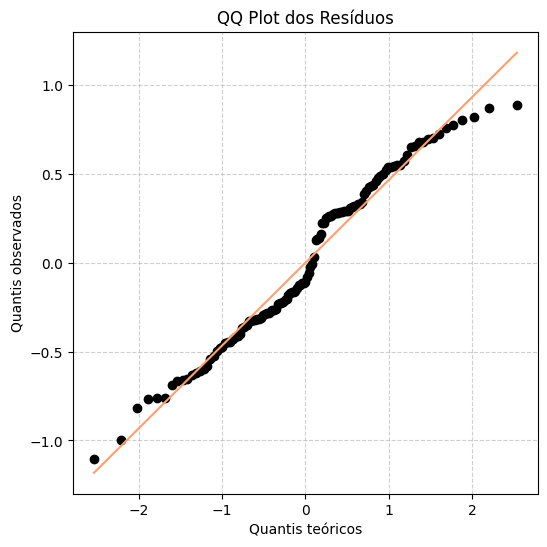
\includegraphics[width=0.55\textwidth]{figuras/centralidade_grafo/qqplot residuos.png}
    }
    \caption{QQ Plot ilustrando a normalidade dos resíduos. Fonte: A própria autora. }
    
\end{figure}
Intuitivamente, a correlação faz sentido, pois quanto mais paradas o sistema tem,  maior é a cobertura da cidade, e menos central cada parada será, dado que cada uma se torna menos crítica para conectar diferentes áreas, caso haja uma boa distribuídas pelo espaço e rotas.


\begin{figure}[H]
    \centering
    {%
        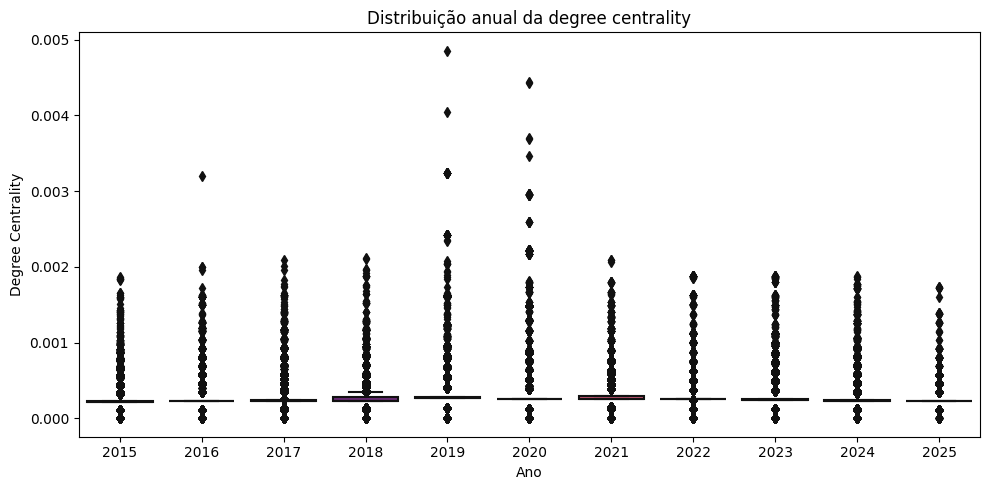
\includegraphics[width=0.85\textwidth]{figuras/centralidade_grafo/degree centrality.png}
    }
    \caption{Boxplots da média de degree centrality por ano. Fonte: A própria autora. }
    
\end{figure}

A distribuição de degree centrality da rede permaneceu praticamente constante ao longo do tempo, indicando que a conectividade das paradas permaneceu estável, ou seja, cada parada mantém aproximadamente o mesmo número de conexões, sem grandes mudanças na estrutura. Notamos apenas alguns outliers a mais em 2017 e 2018, período em que, aparentemente, houve uma reestruturação da rede.

\begin{figure}[H]
    \centering
    {%
        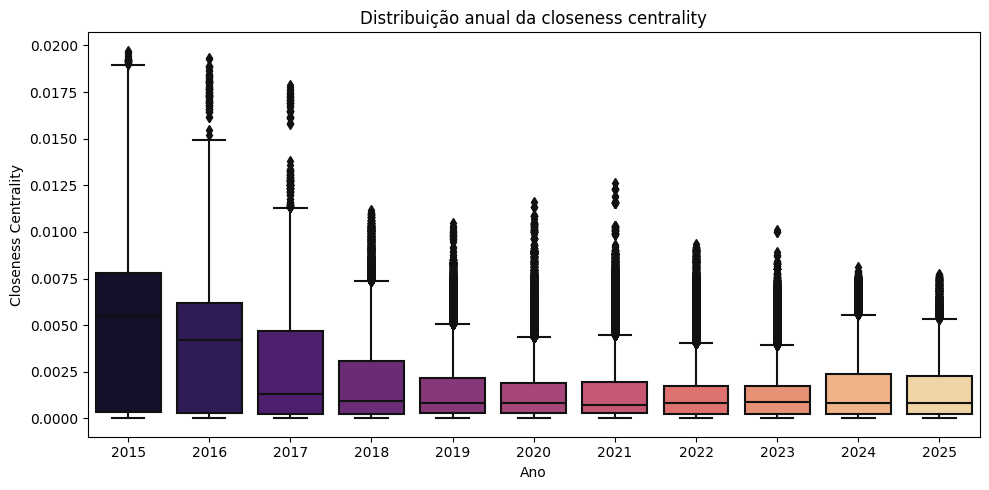
\includegraphics[width=0.85\textwidth]{figuras/centralidade_grafo/closeness.png}
    }
    \caption{Boxplots da média de closeness centrality por ano. Fonte: A própria autora. }
    
\end{figure}

O gráfico mostra que a closeness centrality diminuiu consistentemente ao longo dos anos, indicando que a rede de transporte se tornou menos centralizada. Entre 2015 e 2017, alguns nós eram muito próximos de todos os outros. A partir de 2018, quando suspeitamos ter ocorrido uma reestruturação, os valores ficaram mais baixos e com menos variância, sugerindo que a rede se tornou mais equilibrada, com menor dependência de pontos específicos para conectar o sistema. Essa conclusão é idêntica a que obtivemos ao analisar a métrica de betweenness centrality.

\subsection{Análise geral dos passageiros}

Buscando analisar a distribuição geral da quantidade de pessoas que utilizam o transporte ao longo dos anos, elaboramos algumas visualizações:

\begin{figure}[H]
    \centering
    {%
        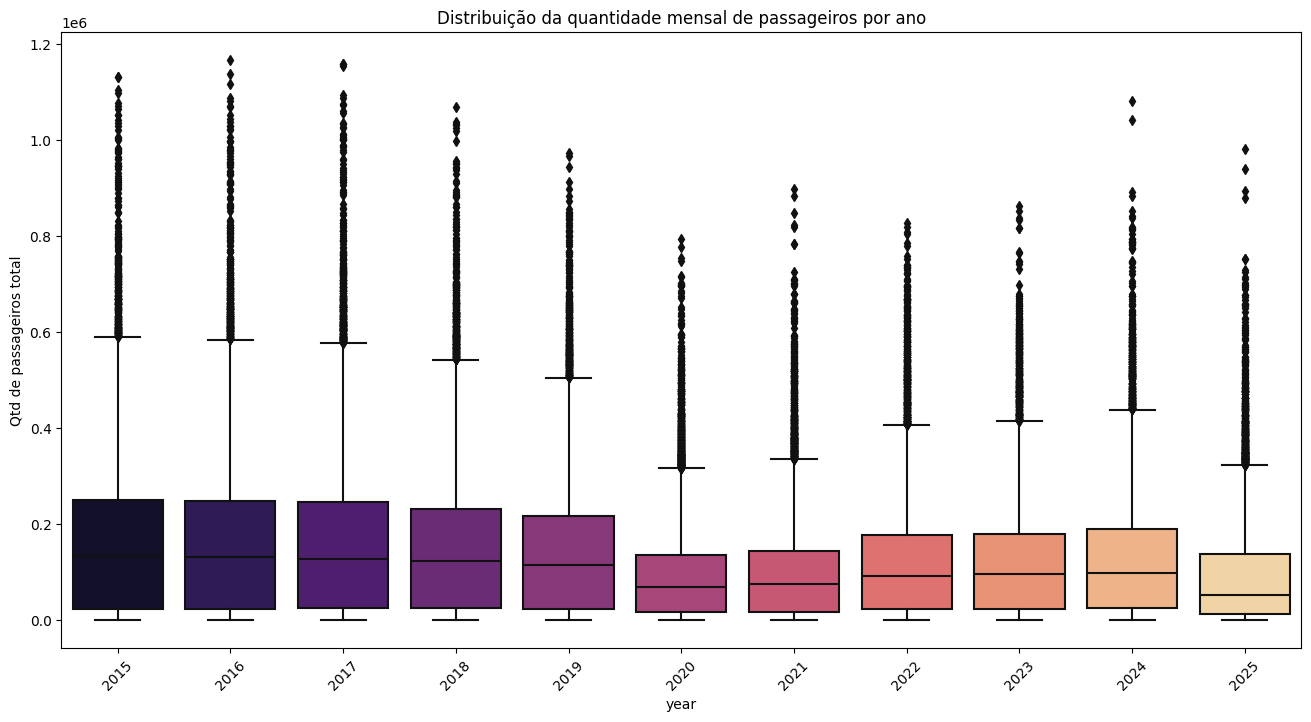
\includegraphics[width=0.85\textwidth]{figuras/passageiros/qtd mensal de passageiros ano.png}
    }
    \caption{Quantidade mensal de passageiros por ano. Fonte: A própria autora. }
    
\end{figure}

A partir do gráfico acima, podemos concluir que a maioria das linhas transporta até 200 mil passageiros por mês, tendo muitos outliers, e que houve uma queda abrupta de passageiros em 2020, sendo que desde então, ano a ano, a quantidade de passageiros tem aumentado, mas ainda está distante do patamar pré pandemia. Desconsideramos 2025 pois ainda não temos dados do ano inteiro.

Como os dados de passageiros são discriminados por várias categorias, podemos tentar visualizar qual o impacto de cada categoria no total de passageiros:

\begin{figure}[H]
    \centering
    {%
        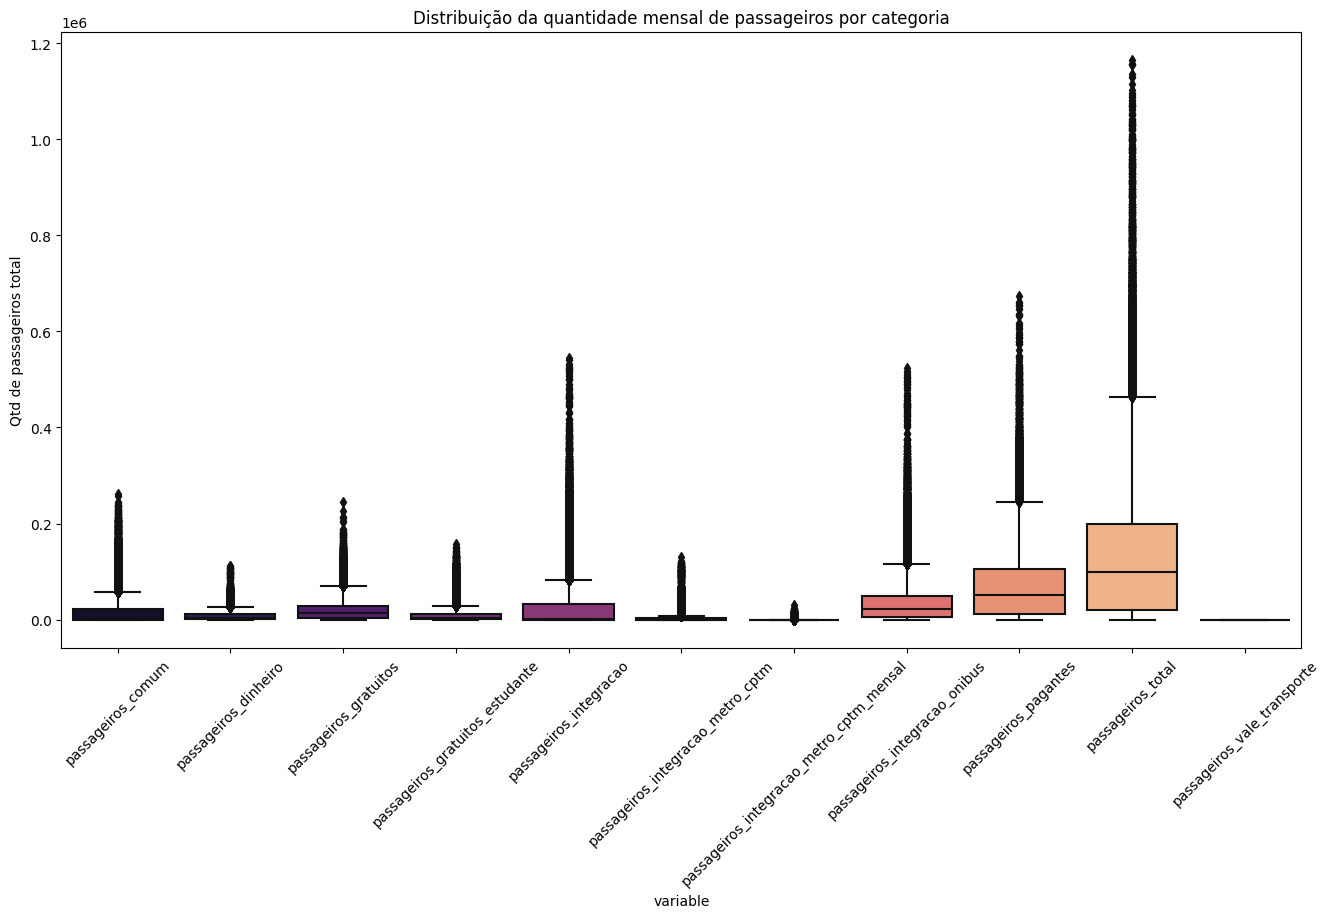
\includegraphics[width=0.85\textwidth]{figuras/passageiros/qtd de passageiros por categoria.png}
    }
    \caption{Quantidade mensal de passageiros por categoria. Fonte: A própria autora. }
    
\end{figure}

Primeiramente, podemos concluir que há algumas inconsistências nos dados: a quantidade de passageiros em vale transporte está zerada, e os dados de passageiros que fazem integração do metrô e CPTM estão mais baixos que o esperado. Tirando essas categorias, podemos notar que há muitos passageiros que fazem integrações entre ônibus (pegando mais que um ônibus para completar o seu trajeto), tendo muitos outliers, e que a maioria dos passageiros é pagante. Para as categorias de passageiros com gratuidade e que pagam com dinheiro vamos elaborar visualizações separadas.

\begin{figure}[H]
    \centering
    {%
        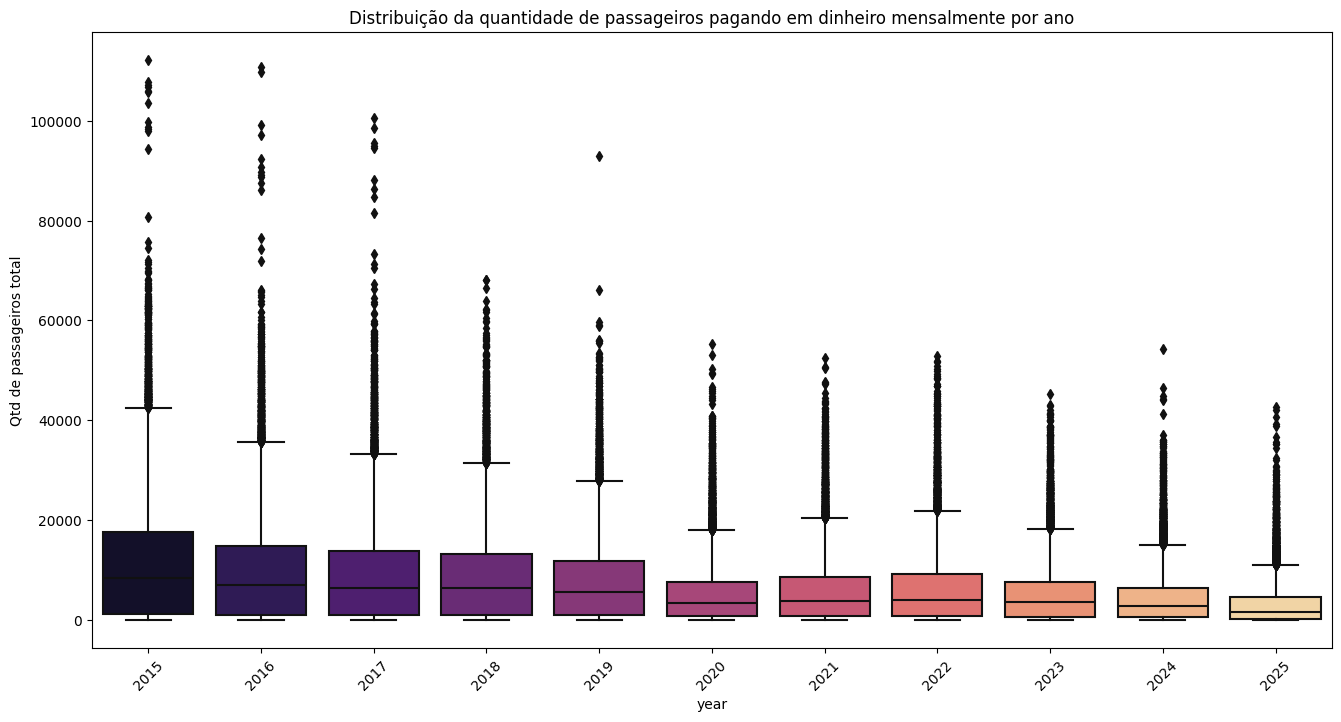
\includegraphics[width=0.85\textwidth]{figuras/passageiros/qtd passageiros dinheiro ano.png}
    }
    \caption{Quantidade mensal de passageiros pagando em dinheiro. Fonte: A própria autora. }
    
\end{figure}

Podemos notar que a quantidade de passageiros que paga em dinheiro vem diminuindo ao longo dos anos, e que temos ausência de dados nas bases.

\begin{figure}[H]
    \centering
    {%
        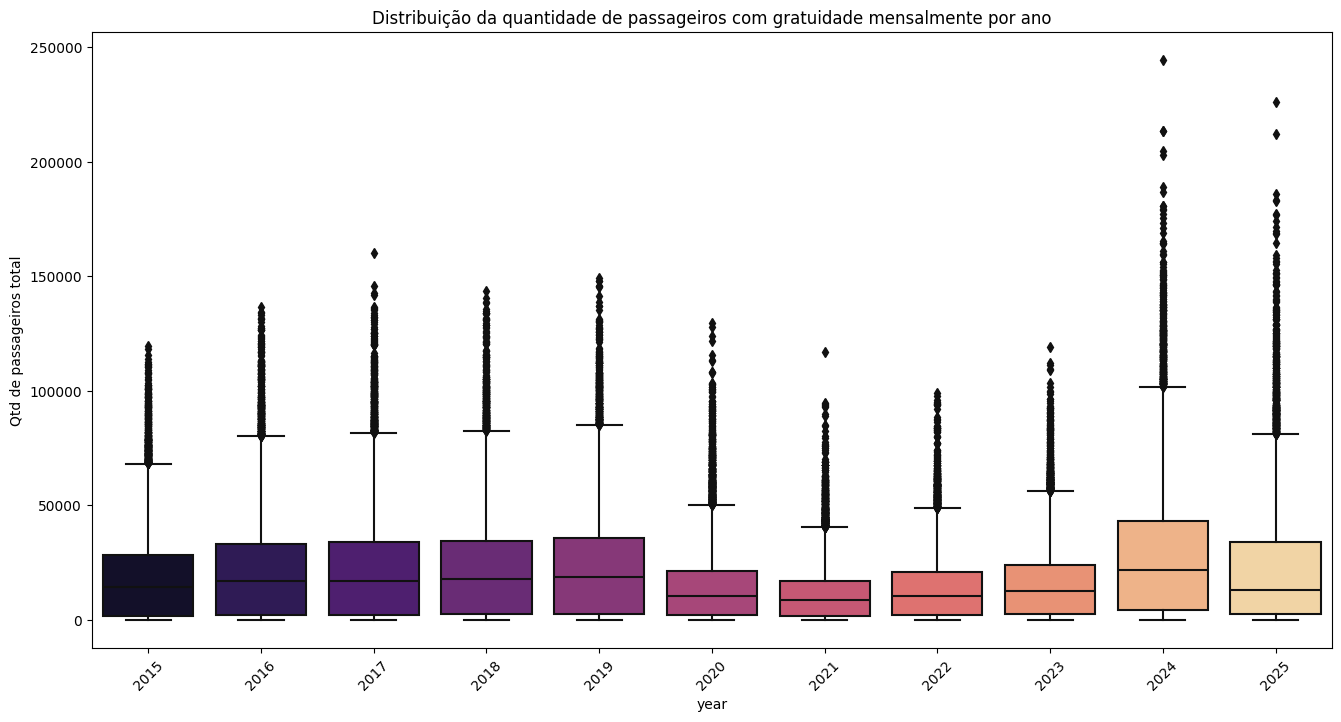
\includegraphics[width=0.85\textwidth]{figuras/passageiros/qtd passageiros gratuitos por ano.png}
    }
    \caption{Quantidade mensal de passageiros com gratuidade. Fonte: A própria autora. }
    
\end{figure}

 Já no gráfico de passageiros com gratuidade, observamos uma queda nos anos de 2020 e 2021, seguida por um aumento em 2024, que apresenta a mediana mais alta de todo o período analisado. Esse resultado indica que, recentemente, mais pessoas têm usufruído da gratuidade no transporte público, sugerindo um avanço nas políticas de inclusão social. 
 
 Podemos procurar entender, junto a própria SPTrans, quais são os motivos para as pessoas receberem a gratuidade, buscando entender se é por questão de renda, idade ou deficiência. Esses dados poderiam, possivelmente, serem utilizados para melhoria das políticas públicas da cidade.

\section{Análise da Reestruturação das Linhas de Ônibus da Zona Oeste após a Inauguração da Estação Vila Sônia}

\subsection{Contexto da Inauguração}
A Estação Vila Sônia, correspondente à última etapa da segunda fase da Linha 4‑Amarela do Metrô de São Paulo, foi inaugurada em 17 de dezembro de 2021 como parte de complexo integrando metrô e terminal de ônibus. Embora aberta ao público nessa data, o terminal operou inicialmente em modo de operação assistida (por exemplo, com horários limitados) e só atingiu funcionamento integral no dia 10 de maio de 2022. 

Após a inauguração de uma estação de metrô nova, é de se esperar que haja um replanejamento das linhas de ônibus que transportam os passageiros naquela região. Nessa seção, vamos ilustrar as mudanças que ocorreram nas linhas após a inauguração da estação, e quais os impactos sociais e econômicos dessa reestruturação. 

\subsection{Seleção das Linhas da Zona Oeste}
Para obtermos as linhas que passam próximas a estação Vila Sônia, utilizaremos o atributo "Estação mais próxima" da tabela de paradas. Mesmo com esse filtro, ainda há linhas que estão na base mas não são nosso alvo de estudos, como as diversas linhas que passam pela Avenida Francisco Morato. Desse modo, vamos expandir nosso filtro para pegar apenas aquelas cujos destinos foram alterados para o terminal Vila Sônia, ou seja, as que contém Vila Sônia no nome da rota.

A partir desses filtros, podemos analisar se houve mudanças significativas nos percursos das rotas entre 2021 e 2025. Essa análise será feita, principalmente, observando a distância percorrida entre os pontos das rotas ao longo dos meses, tomando seus mínimos e máximos. Ao fazer esse cálculo, obtemos a seguinte tabela:

\begin{table}[htbp]
\centering
\resizebox{\textwidth}{!}{%
\begin{tabular}{lrrrl}
\toprule
route\_id & min\_dist\_km & max\_dist\_km & dist\_km & route\_long\_name \\
\midrule
745810 & 6.189507 & 17.096346 & 10.906839 & Jd. Boa Vista - Est. Da Luz, Jd. Boa Vista - Term. Vl. Sônia \\
701310 & 5.684849 & 10.539948 & 4.855099 & Pq. Arariba - Pinheiros, Pq. Arariba - Term. Vl. Sônia \\
807710 & 6.176721 & 9.682711 & 3.505991 & Jd. João Xxiii - Metrô Butantã, Jd. João Xxiii - Term. Morumbi, Jd. João Xxiii - Term. Vl. Sônia \\
807310 & 3.438301 & 6.733491 & 3.295190 & Jd. Guaraú - Butantã, Jd. Guaraú - Term. Morumbi, Jd. Guaraú - Term. Vl. Sônia \\
802310 & 6.945729 & 10.134850 & 3.189122 & Cdhu Munck - Butantã, Cdhu Munck - Term. Morumbi, Cdhu Munck - Term. Vl. Sônia \\
802610 & 5.014927 & 8.091129 & 3.076202 & Jd. Inga - Butantã, Jd. Ingá - Butantã, Jd. Ingá - Term. Vl. Sônia \\
802510 & 3.727406 & 6.657830 & 2.930424 & Jd. Rosa Maria - Butantã, Jd. Rosa Maria - Term. Morumbi, Jd. Rosa Maria - Term. Vl. Sônia \\
801810 & 3.024805 & 4.846033 & 1.821228 & Vl. Sônia - Butantã, Vl. Sônia - Metrô Morumbi \\
807521 & 5.787436 & 7.136091 & 1.348655 & Term. Campo Limpo - Term. Morumbi, Term. Campo Limpo - Term. Vl. Sônia \\
\bottomrule
\end{tabular}%
}
\caption{Distâncias mínimas, máximas e totais por rota. Fonte: A própria autora.}
\label{tab:distancias_rotas}
\end{table}

A partir dessa tabela, podemos notar que muitas das linhas da região tiveram seus caminhos diminuídos. As mais afetadas foram as linhas 745810 e 701310, sendo que ambas ligavam bairros até estações distantes no centro da cidade. O restante das linhas conectava algum bairro até a estação mais próxima, então é de se esperar que, caso surja uma nova estação mais próxima do bairro, o percurso da linha seja alterado até essa estação. 

\subsection{Histórico de passageiros nas linhas afetadas}

Observem, no gráfico abaixo, o histórico de passageiros nas linhas afetadas:

\begin{figure}[H]
    \centering
    {%
        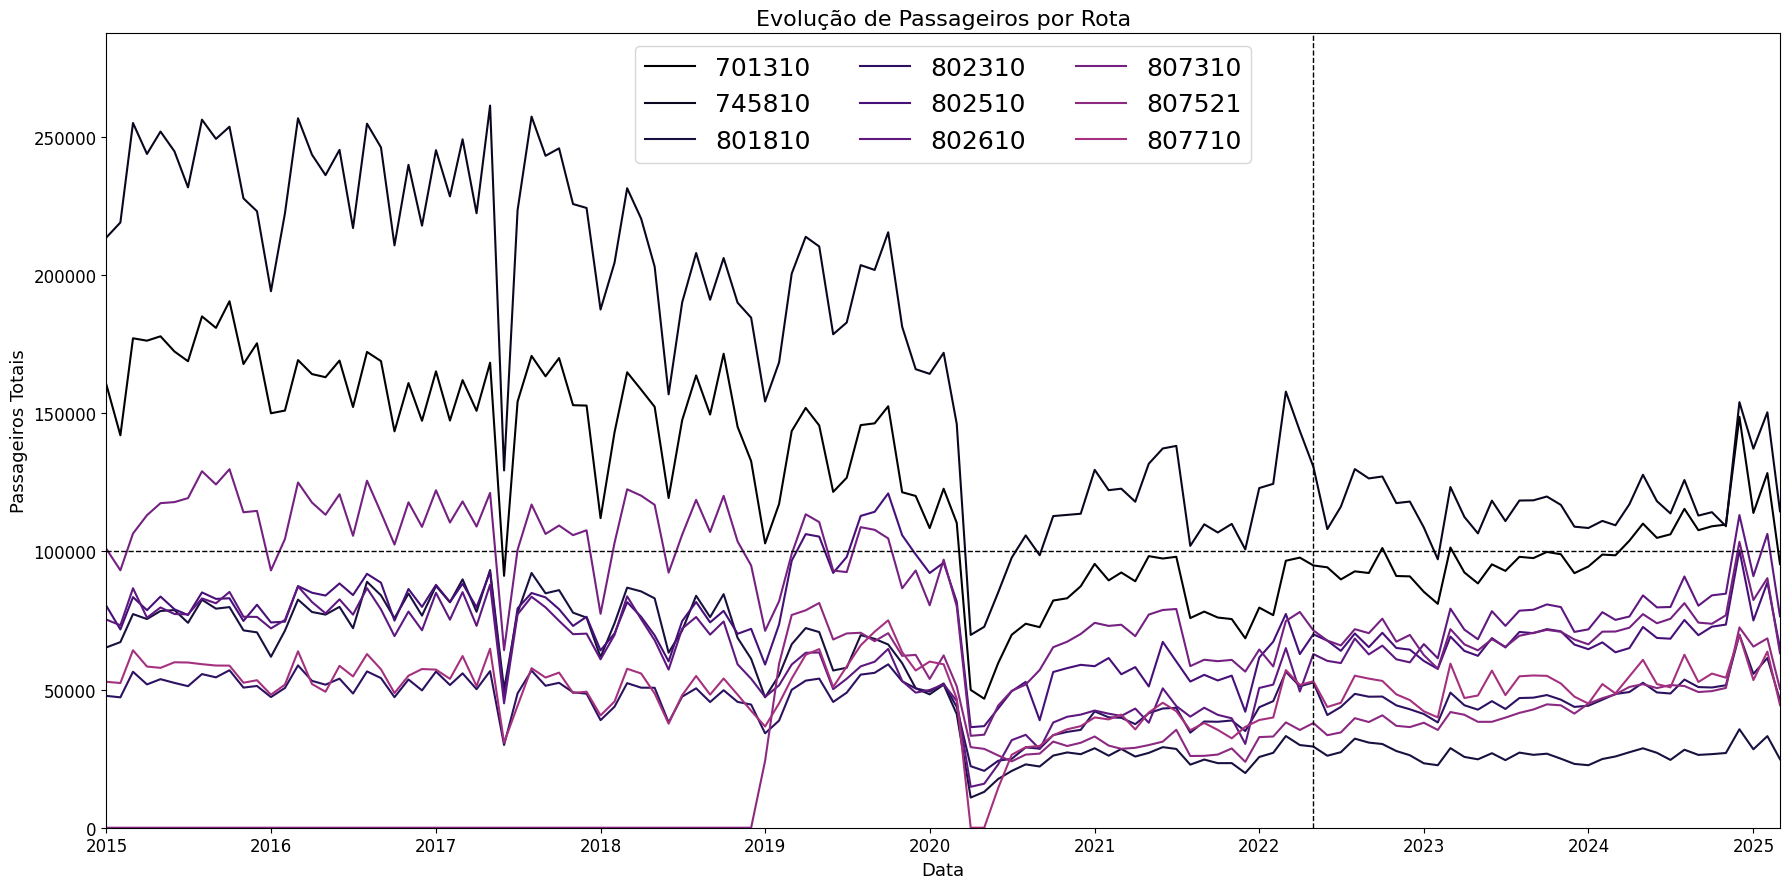
\includegraphics[width=1\textwidth]{figuras/analise_vila_sonia/passageiros rotas afetadas.png}
    }
    \caption{Histórico de passageiros das linhas afetadas mês a mês. Fonte: A própria autora. }
    
\end{figure}
Quando observamos a quantidade de passageiros ao longo dos anos, notamos que todas as rotas sofreram uma queda brusca no número de passageiros no início de 2020. Essa queda coincide com o início da pandemia de COVID-19 e a quarentena em São Paulo. Além disso, após 2020, algumas linhas voltaram a crescer, mas não chegaram a ultrapassar os níveis pré-pandemia. 

Os dados refletem mudanças no comportamento populacional, como home office. Ainda assim, as linhas da região contam com alto número de passageiros transportados, sendo próximas a 100 mil pessoas por mês. Vale notar que as duas linhas mais afetadas em questão de diminuição de quilometragem também são as que mais carregam passageiros na região, o que pode ter motivado a realocação do fluxo dessas rotas para um transporte mais eficiente, como o metrô.

\subsection{As duas linhas mais afetadas: 745810 e 701310}

\subsubsection{A linha 745810}

A linha 745810, que liga o bairro Jd Boa Vista ao centro, foi a mais afetada, saindo de 17km percorridos para apenas 6km. Antes, a linha ia até a Estação da Luz, no centro de São Paulo, passando por pontos importantes como Butantã, Pinheiros, Paulista e República. No gráfico abaixo, é possível observar a drástica mudança no percurso da linha.

\begin{figure}[H]
    \centering
    \subfloat[Rota da linha 745810 Jd Boa Vista - Estação da Luz em mai/2022.]{%
        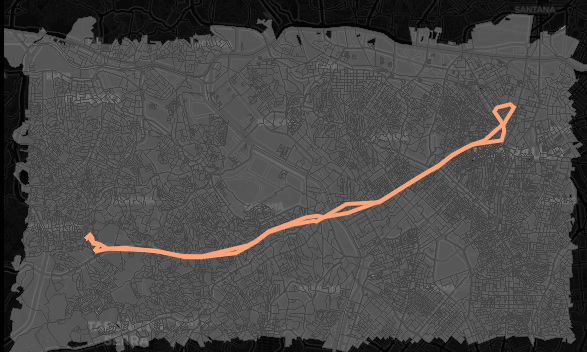
\includegraphics[width=0.45\textwidth]{figuras/analise_vila_sonia/Percurso 745810 mai22.png}
    }
    \hspace{0.05\textwidth}
    \subfloat[Rota da linha 745810 Jd Boa Vista - Term. Vila Sônia em jun/2022]{%
        \includegraphics[width=0.45\textwidth]{figuras/analise_vila_sonia/Percurso 745810 jun22.png}
    }
    \caption{Comparação entre as rotas da linha 745810. Fonte: A própria autora. }
    \label{fig:comparacao}
\end{figure}

Em junho de 2022, a rota foi modificada para ir até a Estação Vila Sônia, o que obriga os passageiros a ou pagar a mais para utilizar o metrô, ou pegar outro ônibus para ir ao seu destino, o que se torna especialmente difícil no horário de pico na Raposo Tavares, por onde passam linhas que ligam bairros dormitórios ao centro. Essas linhas possuem um alto número de passageiros, conforme o boxplot abaixo, que mostra que a média de passageiros nas linhas que passam na região é de 136 mil, e a mediana de 118 mil. 

\begin{figure}[H]
    \centering
    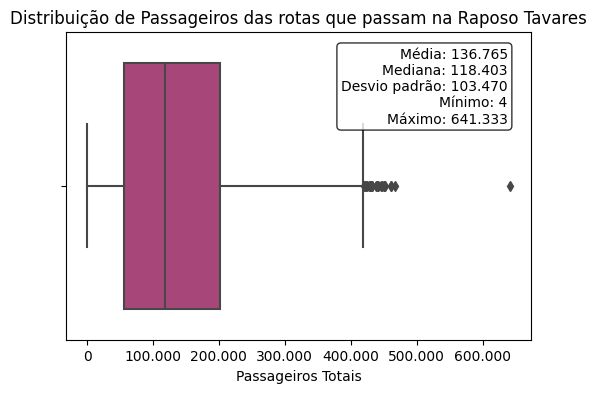
\includegraphics[width=0.7\textwidth]{figuras/analise_vila_sonia/passageiros na raposo tavares.png}
    \caption{Boxplot da quantidade total de passageiros nas linhas que passam pela Raposo Tavares, considerando os 10 anos de dados de passageiros. Fonte: A própria autora.}
    \label{fig:passag_raposo_tavares}
\end{figure}

\begin{figure}[H]
    \centering
    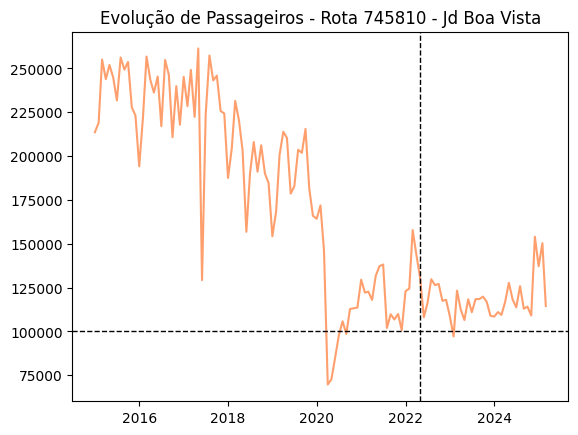
\includegraphics[width=0.6\textwidth]{figuras/analise_vila_sonia/Passageiros rota 745810 - Jd Boa Vista.png}
    \caption{Histórico de passageiros da linha 745810, ao longo de 10 anos. Fonte: A própria autora.}
    \label{fig:passag_745810}
\end{figure}


Segundo o \citet{portal_transito2024}, os ônibus padron possuem capacidade de transportar 80 passageiros. Assumindo que todos os veículos da região seguem esse padrão, para fins de simplificação (há algumas linhas que possuem veículos articulados, mas iremos desconsiderar esses casos), seriam necessários 1875 veículos para transportar as 150 mil pessoas que utilizaram a linha 745810 em dez/24, ou seja, 1 ônibus a cada 4,61 minutos, sabendo que os veículos circulam de 4h40 à 00h00. 

\begin{equation*}
    \frac{60\,\text{minutos} \times 20{,}6\,\text{horas} \times 7\,\text{dias}}{1875\,\text{veículos}} = 4{,}61\,\text{minutos/ônibus}
\end{equation*}

Quando olhamos apenas para os dias úteis, o número de passageiros cai para 119.725 (representando 79.8\% do total), e o número de veículos cai para 1497, ou seja, 1 ônibus a cada 4,12 minutos, ainda erroneamente assumindo que todos os horários do dia possuem o mesmo fluxo.

\begin{equation*}
    \frac{60\,\text{minutos} \times 20{,}6\,\text{horas} \times 5\,\text{dias}}{1497\,\text{veículos}} = 4{,}12\,\text{minutos/ônibus}
\end{equation*}

Segundo os dados do GTFS de março de 2025, na linha 745810, durante os dias de semana, entre 05h e 10h, e 16h e 00h, os ônibus saem com intervalos de 30 minutos, e entre 10h e 16h, com intervalo de 20 minutos. Mesmo assumindo que a maioria dos veículos da rota sejam articulados, com o dobro da capacidade de passageiros (chegando a 160), é possível notar que há demanda em excesso para a quantidade de veículos na frequência proposta. 

De acordo com o censo de 2022, do IBGE, há cerca de 117.738 pessoas que moram no distrito Raposo Tavares, por onde a linha 745810 faz todo o seu trajeto, porém, é importante notar que nos arredores do bairro Jd Boa Vista estão surgindo diversos condomínios prediais do projeto "Reserva Raposo", sendo 22 mil apartamentos planejados, que servirão de moradia para mais de 80 mil pessoas, o que deverá aumentar a demanda da região por transporte. 

\begin{figure}[h]
    \centering
    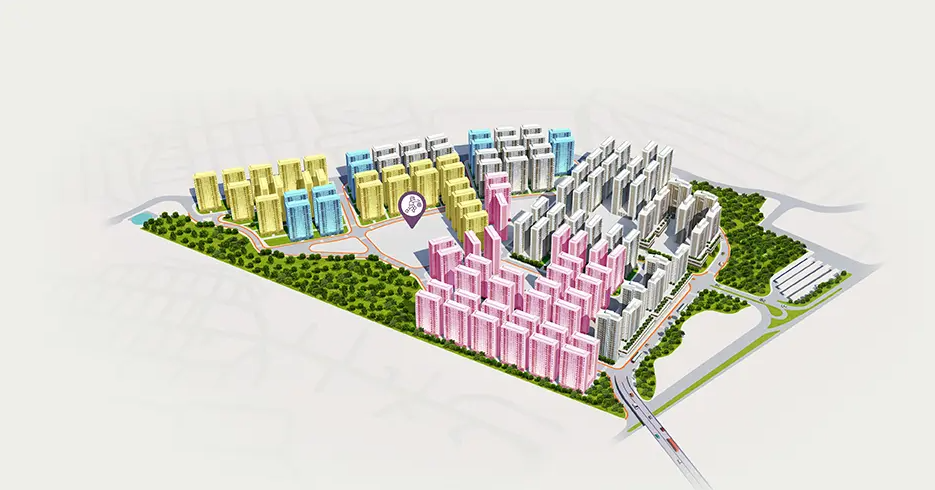
\includegraphics[width=0.8\textwidth]{figuras/analise_vila_sonia/reserva raposo planejamento.png}
    \caption{Plano de construção do Reserva Raposo, um mega projeto de habitação que está sendo construído próximo a Raposo Tavares. Fonte: Reserva Raposo.}
    \label{fig:reserva_raposo}
\end{figure}

Parte da linha 745810 já foi desviada para cobrir algumas paradas próximas aos novos condomínios, porém, no patamar atual, a sobrecarga do sistema é iminente, ainda mais considerando a volta ao trabalho presencial \citep{volta_presencial}. O empreendimento prevê a construção de um terminal rodoviário para dar vazão aos moradores, projeto que poderá ser analisado futuramente, quando novos dados forem disponibilizados.

Desse modo, conseguimos analisar que a nova estação Vila Sônia impactou fortemente os habitantes da região do bairro Jd Boa Vista, que precisaram alterar seus caminhos para chegar ao centro de São Paulo. Apesar de mais rápido e confortável, o metrô cobra uma passagem adicional pelo uso, sem integração tarifária completa com os ônibus da região, o que pode representar um alto impacto no orçamento das famílias, especialmente as de baixa renda. Ao considerarmos que o mega projeto Reserva Raposo é destinado a habitação social, o número de pessoas impactadas fica ainda maior. Esse cenário aponta para a necessidade urgente de revisão da política tarifária da integração ônibus-metrô nas estações inauguradas recentemente, a exemplo do modelo implementado entre os usuários dos ônibus operados pela SPTrans, que podem fazer integração gratuita em uma janela específica ao pagar com o bilhete único. 

Além da questão tarifária, os dados do GTFS indicam que a frequência atual das linhas da região é insatisfatória diante da demanda observada, o que já causa superlotação, problema que tende a se agravar de forma crítica com o projeto Reserva Raposo. Diante disso, recomenda-se que a SPTrans e a Secretaria Municipal de Mobilidade e Transportes adotem a revisão imediata da frequência da linhas 745810 com base nos dados reais de demanda aqui apresentados e a elaboração de um plano de expansão do sistema de transporte para a região, com aprovação em consulta pública com a população da região.

\subsubsection{A linha 701310}

Podemos replicar a mesma análise feita com a linha 745810 para a 701310. A linha 701310 foi a segunda mais afetada pela nova estação, tendo o seu percurso cortado pela metade, alterado de Pinheiros para Vila Sônia. De metrô, esse percurso leva por volta de 15 minutos, porém, novamente, um dos grandes problemas com a reestruturação é o fato do passageiro ter que pagar a mais para trocar de meio de transporte: ou ele paga a mais, ou dificulta seu trajeto pegando um segundo ônibus, o que pode ser difícíl em horário de pico. Esse é mais um cenário que reforça a necessidade da revisão da política de integração entre os transportes da cidade.

A linha 701310 passa pela Estrada do Campo Limpo e Francisco Morato, duas vias importantes para a região. Ao considerarmos todas as linhas que passam pelas duas vias, obtemos os seguintes boxplots:

\begin{figure}[H]
    \centering
    \subfloat[Boxplot da quantidade de passageiros nas linhas da Francisco Morato ao longo de 10 anos]{%
        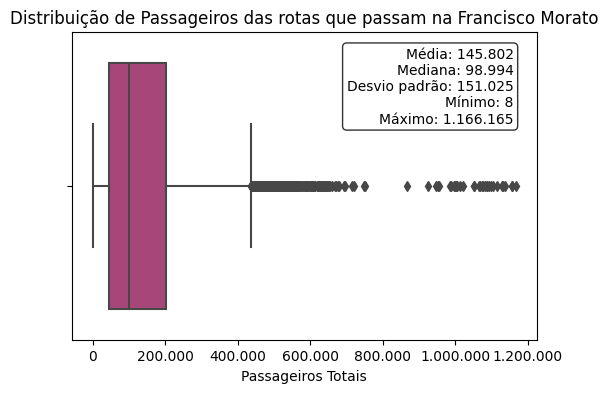
\includegraphics[width=0.7\textwidth]{figuras/analise_vila_sonia/boxplot francisco morato.png}
    }
    \hspace{0.01\textwidth}
    \subfloat[Boxplot da quantidade de passageiros nas linhas da Estrada do Campo Limpo ao longo de 10 anos]{%
        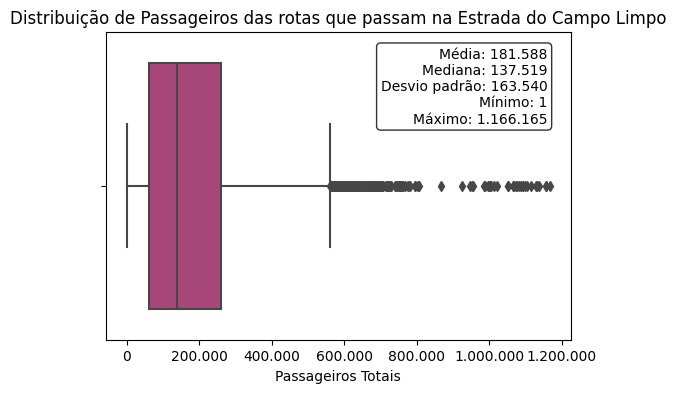
\includegraphics[width=0.7\textwidth]{figuras/analise_vila_sonia/boxplot estrada campo limpo.png}
    }
    \caption{Comparação entre os boxplots da quantidade de passageiros nas principais vias da linha 701310. Fonte: A própria autora. }
    \label{fig:comparacao}
\end{figure}



Nesses gráficos, é possível notar que a quantidade de passageiros nos ônibus das duas regiões é tão alta quanto as da Raposo Tavares. Vale notar que, nesses dados, temos máximos muito maiores do que no boxplot da Raposo Tavares. Temos aqui, então, o mesmo problema de transferência entre ônibus

Observe, no gráfico abaixo, que a quantidade de passageiros da linha 701310 fica próxima de 100 mil pessoas, após a pandemia. Se considerarmos os dados de passageiros de dezembro de 2024, maior pico dos últimos meses, temos que, para transportar 148,71 mil passageiros no mês, seriam necessários um ônibus padron a cada 4,61 minutos, ou um ônibus articulado a cada, aproximadamente, 9 minutos, diferindo muito do horário atual da linha que, entre 06h-07h e 07h-08h, tem uma frequência de 1 ônibus a cada 30 minutos. Vale notar que, para esse cálculo, consideramos que a linha opera por 20,6 horas, mas na verdade, ela também opera entre 00h e 2h da manhã, tendo um horário de operação total de 21,63 horas. Optamos por desconsiderar esse período adicional na operação, dado que a quantidade de passageiros nas linhas noturnas exclusivamente noturnas não é alta.

\begin{figure}[H]
    \centering
    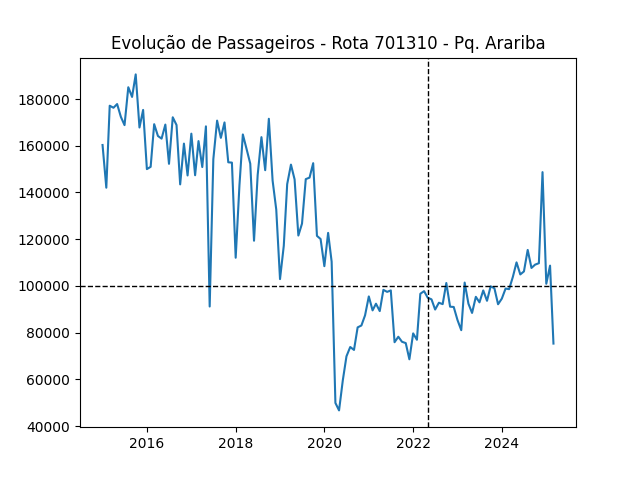
\includegraphics[width=0.6\textwidth]{figuras/analise_vila_sonia/Passageiros rota 701310 - Pq. Arariba.png}
    \caption{Histórico de passageiros da linha 701310, ao longo de 10 anos. Fonte: A própria autora.}
    \label{fig:passag_701310}
\end{figure}

\subsubsection{Outras considerações}

As linhas Jd João XXIII, Jd Guaraú, CDHU Munck, Jd Ingá e Jd Rosa Maria também foram afetadas, porém em um grau menor do que as outras duas: seus percursos foram redirecionados do Butantã para a estação Morumbi e, posteriormente, para a Vila Sônia. Apesar de parecer ter menos impacto, essa mudança afetaria com muito mais peso, por exemplo, estudantes da USP Butantã que moram nesses bairros e foram forçados a ou fazer um trajeto mais difícil e demorado, pegando um segundo ônibus, ou pagando a mais pelo metrô.

\section{Painel interativo - Analise qualquer rota da cidade da SPTrans}

Vendo como pode ser importante analisar uma rota específica detalhadamente, desenvolvemos um dashboard interativo para explorar informações históricas e operacionais das rotas de transporte público de São Paulo. O painel centraliza diferentes bases, incluindo dados de passageiros, frequências, distâncias percorridas e um mapa com o trajeto, para cada linha de ônibus. 

O usuário pode selecionar uma rota específica em um menu suspenso, que atualiza automaticamente todas as visualizações e tabelas exibidas, permitindo ao usuário analisar e comparar o comportamento e a evolução de cada linha, observando métricas como volume de passageiros, distância total da rota, distância realmente percorrida e frequência programada ao longo dos anos. 

\begin{figure}[H]
    \centering
    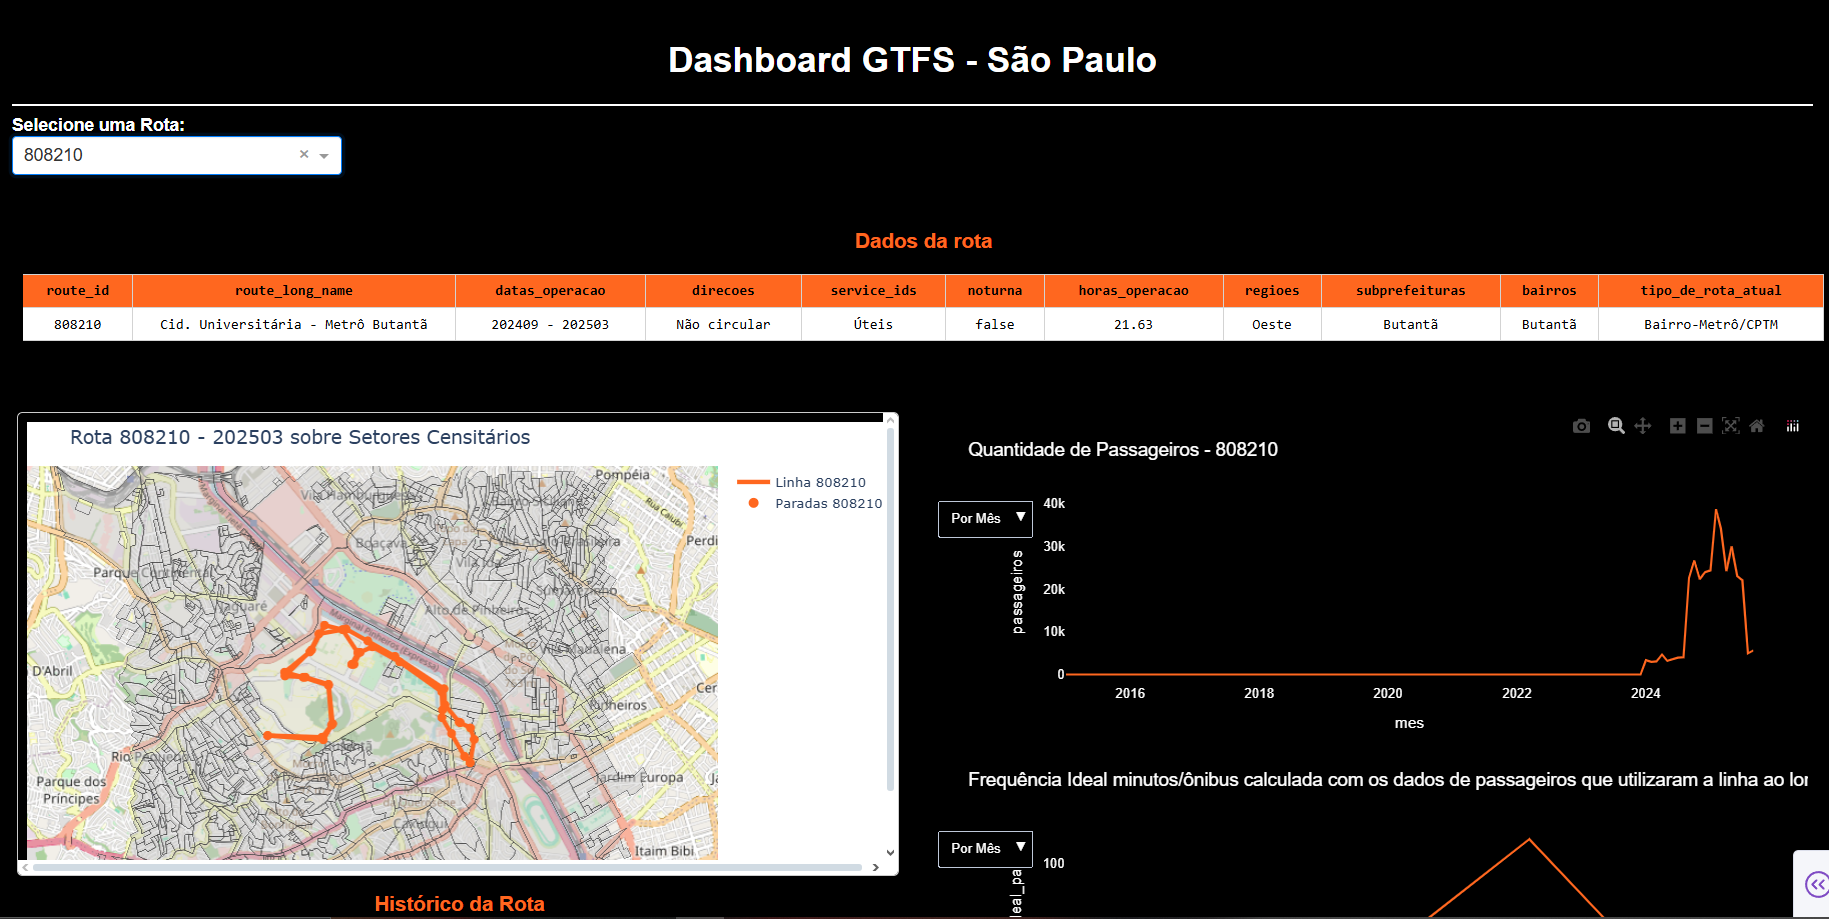
\includegraphics[width=1\textwidth]{figuras/print dash 1.png}
    \caption{Captura de tela do dashboard interativo, com a rota 808210 selecionada no filtro, ilustrando a seção resumo dos principais dados da rota, o histórico mais recente da rota e a série temporal da quantidade de passageiros. Fonte: A própria autora.}
    
\end{figure}

\begin{figure}[H]
    \centering
    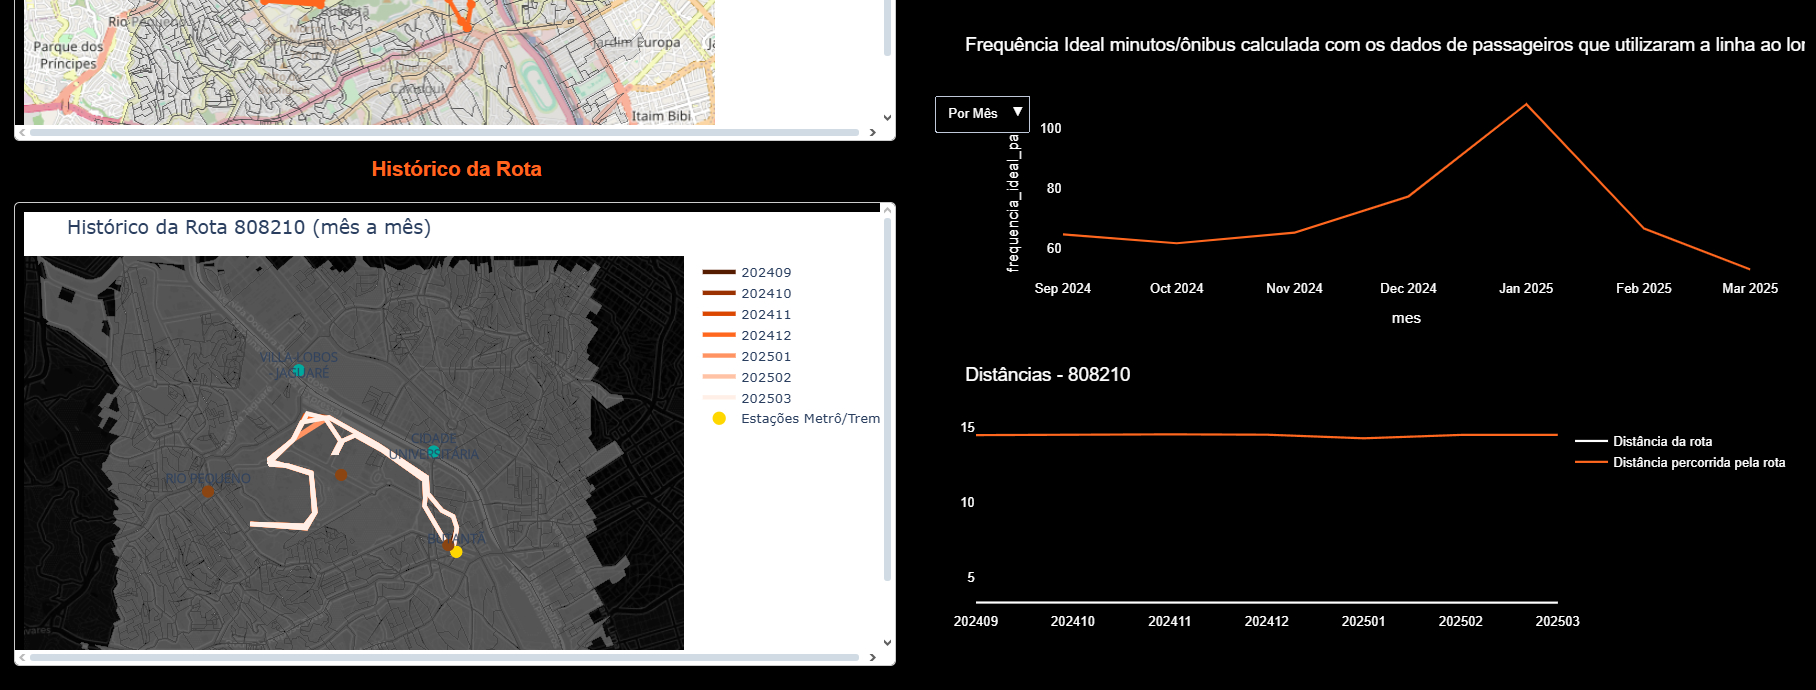
\includegraphics[width=1\textwidth]{figuras/print dash 2.png}
    \caption{Captura de tela do dashboard interativo, com a rota 808210 selecionada no filtro, ilustrando a seção de histórico da rota, frequência ideal calculada e distância percorrida. Fonte: A própria autora.}
    
\end{figure}

O dashboard foi desenvolvido para que os cidadãos possam observar a rota que mais utilizam de forma mais detalhada, e obter dados que auxiliem seus pedidos de melhoria. Por exemplo, ao analisarmos que a frequência ideal de uma rota é muito menor do que a frequência atual, podemos pedir o aumento da frequência para as autoridades competentes, utilizando-se de dados que mostrem a quantidade real de passageiros que se utilizam da rota.

O dashboard está disponível no repositório do trabalho, e pode ser executado através do arquivo app\_rotas.py. 

% O dashboard foi hospedado no Render, com o hosting dos datasets no Hugging Face, estando disponível através do site \url{}

\section{Resumo dos principais resultados e suas interpretações}





\begingroup
\small % reduz o tamanho da fonte

\begin{longtable}[c]{
  p{0.45\textwidth}
  p{0.45\textwidth}
}

\toprule
\makecell{\textbf{Resultado}} &
\makecell{\textbf{Implicações}} \\
\midrule
\endfirsthead

\toprule
\makecell{\textbf{Principal resultado}} &
\makecell{\textbf{Implicações}} \\
\midrule
\endhead

\multicolumn{2}{r}{\textit{continua}\enspace$\longrightarrow$} \\
\caption[]{Quadro de principais achados e implicações da pesquisa.}
\endfoot

\bottomrule
\caption[]{Quadro de principais achados e implicações da pesquisa. Fonte: A própria autora.}
\endlastfoot

\captionlistentry{Quadro de principais achados e implicações da pesquisa.}\label{tab:achados-implicacoes}

% ===================== CONTEÚDO ===================== %
\textbf{Reestruturação do sistema de transporte} \\
O número de paradas cresceu continuamente, enquanto o de rotas diminuiu até 2020 e só então voltou a crescer. &
A rede expandiu sua cobertura física e passou por forte reestruturação durante a pandemia. \\

Zonas Sul e Leste concentram o maior número total de paradas e rotas. &
A oferta reflete a extensão territorial e a alta demanda populacional dessas regiões. \\

Zonas Oeste e Centro se destacam na criação de novas rotas, sem aumento proporcional de paradas. &
O planejamento tem sido mais intenso nessas áreas, priorizando reestruturação e eficiência. Considerando que há migração de empregos para outras zonas da cidade, as zonas com prioridade no planejamento podem ser revisadas.  \\

\midrule
\multicolumn{2}{l}{\textbf{Correlação com a População}} \\
Correlação positiva forte entre número de paradas e população afetada. &
A expansão das paradas tem sido eficiente, priorizando áreas mais populosas. \\

\midrule
\multicolumn{2}{l}{\textbf{Análise de Centralidade da Rede}} \\
As métricas de centralidade (betweenness e closeness) caíram após 2018. &
A rede tornou-se menos centralizada e mais distribuída, reduzindo a dependência de poucos nós. \\

Correlação negativa entre centralidade e número de paradas. &
Com mais paradas, cada ponto torna-se menos crítico para o funcionamento geral. \\

\midrule
\multicolumn{2}{l}{\textbf{Características e Rankings das Rotas}} \\
Rotas com mais passageiros (ex: Itaquera, Jd. Ângela) ligam bairros periféricos a áreas centrais. &
Evidencia o papel essencial dessas linhas na conexão entre periferias e polos de emprego. \\

Itaquera tem muitas paradas e poucas linhas longas (média de 27,5 km). &
O bairro possui rotas extensas e sobrecarregadas; um replanejamento poderia reduzir tempos e melhorar o serviço. \\

Jardim Ângela lidera em número de rotas e paradas próximas, com alta demanda. &
A futura estação de metrô deve reduzir significativamente o tempo de viagem e aliviar a rede. \\

\midrule
\multicolumn{2}{l}{\textbf{Perfil e Volume de Passageiros}} \\
Houve queda abrupta em 2020 (pandemia); a recuperação é parcial. &
A pandemia alterou padrões de mobilidade e comportamento (ex: home office). \\

Pagamento em dinheiro vem diminuindo. &
Indica maior adesão ao Bilhete Único e à digitalização dos pagamentos. \\

Aumentou o número de passageiros com gratuidade em 2024. &
Reflete expansão de políticas de inclusão social e maior acesso ao transporte. \\

\midrule
\multicolumn{2}{l}{\textbf{Reestruturação da Zona Oeste (Estação Vila Sônia)}} \\
\addlinespace[3pt]
A inauguração da Estação Vila Sônia (2022) levou à reestruturação de linhas que iam ao centro. &
O sistema migrou para modelo integrativo (ônibus + metrô), reduzindo tempo, mas elevando custos. \\

O encurtamento de linhas obriga nova tarifa ou baldeações. &
Gerou impacto financeiro e de tempo para os passageiros, especialmente nas linhas mais cheias, o que reforça a necessidade de revisão da política de integração entre os transportes. \\

A linha 745810 (Jd. Boa Vista) transporta ~150 mil passageiros/mês, com frequência insuficiente. &
A oferta é criticamente menor que a demanda; há risco de colapso com o crescimento regional. Há necessidade urgente de revisão da frequência da linha. \\

\midrule
\multicolumn{2}{l}{\textbf{Ferramenta de Análise (Dashboard)}} \\*
Foi desenvolvido um painel interativo para consulta pública. &
Promove transparência e empodera cidadãos a demandar melhorias baseadas em dados. \\

\end{longtable}
\endgroup





% --- Fim do Quadro (longtable) ---

